%Autor: Aarón Martín Castillo Medina.
%Asesora: Dra. Katya Rodríguez Vázquez.
%Contacto: katya.rodriguez@iimas.unam.mx; amcm329@hotmail.com

%En este archivo se conjuntan las partes que conforman la tesis, además
%se introducen algunas directivas para personalizar el comportamiento del
%trabajo para determinadas secciones.


%Aquí se indica que la tesis consta de un reporte a dos páginas con
%letra de tamaño 12.
\documentclass[12pt,twoside]{report}

%Este paquete permite la carga adecuada de subarchivos .tex, respetando
%(con ayuda de la opción subpreambles=true) los paquetes cargados en cada
%subarchivo.
\usepackage[subpreambles=true]{standalone}

%Se cargan todos los paquetes que se encuentran en packages_used.sty
\usepackage{packages_used_standard}

%Aquí se le indica al documento que el número máximo de secciones anidadas 
%toleradas es 4, esto sobre todo tiene repercusiones en el Apéndice.
\setcounter{secnumdepth}{4}

%Para agregar una nueva pagina en blanco sin que se
%recorra el contenido que se encuentre en páginas posteriores.
\newcommand\blankpage{%
                      \null
                      \thispagestyle{empty}%
                      \addtocounter{page}{-1}%
                      \newpage
                     }

%Para ajustar los colores de los hipervínculos.
\hypersetup{
            colorlinks = true,
            linkcolor = black,
            filecolor = magenta,      
            urlcolor = cyan
           }
 
%Aquí se indica la ruta de las imágenes que se utilizarán en la tesis.
\graphicspath{ 
              {images/}
             }

%Se modifica el "Indice General" para que en su lugar se escriba
%"Tabla de Contenido".
\addto\captionsspanish{
                       % Reemplazar "spanish" con el lenguaje que se usa
                       \renewcommand{\contentsname}%
                       {Tabla de Contenido}%
                      }

%Por defecto al inicio de cada capítulo aparece "Chapter N", entonces
%con esta instrucción se elimina ese espacio por defecto.
%\titleformat{\chapter}[display]{\normalfont\bfseries\centering}{}{0pt}{\LARGE}

%Se modifica el formato de todas las secciones de la tesis.
\titleformat*{\section}{\Large\bfseries}

%Se modifica el formato de todos los capítulos de la tesis.
\titleformat{\chapter}[display]{\normalfont\huge\bfseries}{\chaptertitlename\ \thechapter}{11pt}{\Huge}

%Las siguientes líneas corresponden a la información que se 
%mostrará en el encabezado de las páginas.
%A la izquierda de cada página par se mostrará el texto 
%"No. Página - Capítulo No. X"
\fancyhead[LE]{\textbf{\thepage}\ \ \ \ Capítulo\ \thechapter}

%A la derecha de cada página par no se mostrará nada.
\fancyhead[RE]{}

%A la izquierda de cada página impar no se mostrará nada.
\fancyhead[LO]{}

%A la derecha de cada página impar se muestra la información 
%"Nombre del capítulo - No. Página"
\fancyhead[RO]{\leftmark \ \ \ \ \textbf{\thepage}}

%A continuacipón se contemplan las características que tendrá
%el pie de las páginas.
%Con esta línea se coloca un margen en la parte inferior para
%identificar al pie de página.
\renewcommand{\footrulewidth}{0.4pt}% default es 0pt

%En la parte izquierda del pie de página (sin importar si es par 
%o impar) se pondrá la palabra "UNAM".
\lfoot{UNAM}

%En la parte derecha del pie de página (sin importar si es par 
%o impar) se pone la palabra "Facultad de Ciencias".
\rfoot{Facultad de Ciencias}

%Enla parte centro del pie de página (sin importar si es par 
%o impar) se coloca un espacio vacío.
\cfoot{}

%Se comienzan a integrar las partes de la tesis.
\begin{document}

       %Se inserta la portada que se encuentra en el archivo cover.tex.
       %Autor: Aarón Martín Castillo Medina.
%Asesora: Dra. Katya Rodríguez Vázquez.
%Contacto: katya.rodriguez@iimas.unam.mx; amcm329@hotmail.com

%Este archivo permite elaborar la portada y por ende el título de 
%la obra; además se incluyen elementos adicionales como información 
%básica del autor,nombre completo de la asesora, incluso se proyectan 
%imágenes con los escudos tanto de la U.N.A.M como de la Facultad de 
%Ciencias.       


%Se indica que el documento es de tipo reporte bajo el paquete standalone.
\documentclass[class=report, crop=false]{standalone}

%Se cargan todos los paquetes que residen en el archivo packages_used_standard.sty
\usepackage{packages_used_standard}

%Comienza el documento.
\begin{document}

%Es menester colocar estas directivas alusivas al título y a la 
%fecha para que éstas se puedan colocar en otras secciones de la 
%portada y no cause errores en la distribución de elementos.
\title{}
\date{}

%Se coloca esta directiva para eliminar encabezado y pie de 
%página.
\thispagestyle{empty}

%Se hace un recorrido horizontal a la izquierda para centrar 
%la portada.
\hskip+0.2cm
%La portada se divide en dos secciones, a continuación se trata
%la primera sección que consiste en los escudos tanto de la U.N.A.M.
%y la Facultad de Ciencias, además de las franjas horizontales.
\begin{minipage}[c][10cm][s]{3cm}
      %Se coloca este espacio para ajustar esta sección adecuadamente
      %de manera vertical para que no haya mucho espacio debajo.
      \vspace{-1.2cm}
      %Todo el contenido de esta sección se pasa a la 
      %izquierda.
      \flushleft
      
      %Se coloca y centra el escudo de la U.N.A.M.
      \center{
\includegraphics[width=2.8cm,height=2.9cm]{images/unam.pdf}}
      
      %Se adjunta un espacio entre el escudo y las franjas.
      \vspace{0.7cm}
 
      %Se ponen las 3 franjas verticales.
      \center{
              \vrule width.5pt height15cm\hskip5mm
              \vrule width2pt height15cm\hskip5mm
              \vrule width.5pt height15cm
             } \\

      %Se agrega un espacio entre las franjas y el otro escudo.
      \vspace{0.5cm}

      %Se añade y centra el escudo de la Facultad de Ciencias.
      \center{
\includegraphics[width=3.0cm,height=3.1cm]{images/ciencias.pdf}}

\end{minipage}
%Se añade este espacio para separar adecuadamente las dos franjas 
%horizontales con el escudo de la U.N.A.M.
\hspace{0.6cm}
%Termina la primera sección.
%No se debe quitar el espacio entre las secciones porque eso 
%repercute en la portada.
%La segunda sección contiene toda la información adicional de la portada.
\begin{minipage}[c][9.7cm][s]{9.9cm}
      %Se coloca este espacio para ajustar esta sección adecuadamente
      %de manera vertical para que no haya mucho espacio debajo.
      \vspace{-1.2cm}
      %Todo el contenidd de esta sección se mueve a la derecha.
      \flushright   
   
      %Se centran los nombres de la Universidad, las franjas horizontales
      %y la Facultad.
      \center{              
              %Se hace una reducción de espacio vertical para que el nombre
              %de la Universidad esté en el mismo renglón que el inicio del
              %escudo de la U.N.A.M.
              %\vspace{-0.8cm}

              %Se crea y centra el nombre de la Universidad.
              \center{
                      {\fontsize{16pt}{16pt}\selectfont U}{\fontsize{13pt}{13pt}\selectfont NIVERSIDAD} {\fontsize{16pt}{16pt}\selectfont N}{\fontsize{13pt}{13pt}\selectfont ACIONAL} 
                      {\fontsize{16pt}{16pt}\selectfont A}{\fontsize{13pt}{13pt}\selectfont UTÓNOMA} \\[6pt]
                      {\fontsize{13pt}{13pt}\selectfont DE} 
                      {\fontsize{16pt}{16pt}\selectfont M}{\fontsize{13pt}{13pt}\selectfont ÉXICO} 
                     } \\

              %Se crean las dos franjas horizontales.   
              \vspace{0.3cm}
              \hrule height2pt\hspace{15pt}
              \vspace{0.5cm}
              \hrule height.5pt\hspace{15pt}	
              \vspace{0.8cm}
          
              %Se inicia con el nombre de la Facultad.
              {\fontsize{16pt}{16pt}\selectfont F}{\fontsize{13pt}{13pt}\selectfont ACULTAD DE } {\fontsize{16pt}{16pt}\selectfont C}{\fontsize{13pt}{13pt}\selectfont IENCIAS}\\[2.0cm]
   
              %Se agrega el nombre de la tesis.
              %\large{\scshape \rmfamily Algoritmos Evolutivos Multiobjetivo y Evaluadores de Desempeño a Través de un Producto de Software  }\\[1.7cm]
              \uppercase{\large{A}\normalsize{lgoritmos} \large{E}\normalsize{volutivos} \large{M}\normalsize{ultiobjetivo y} \large{E}\normalsize{valuadores de} \large{D}\normalsize{esempeño a} \large{T}\normalsize{ravés de un} \large{P}\normalsize{roducto de} \large{S}\normalsize{oftware}}\\[1.8cm]

              %Se escribe la palabra "TESIS" separada por espacios de 1 cm.
              \Huge{T \hspace{1cm} E \hspace{1cm} S \hspace{1cm} I \hspace{1cm} S  }\\[1.6cm]
 
              %Se pone la frase "QUE PARA OBTENER EL TÍTULO DE:".
              \normalsize{QUE PARA OBTENER EL TÍTULO DE:}\\[1.5cm]

              %Se añade la frase "Licenciado en Ciencias de la Computación".
              \normalsize{\uppercase{Licenciado en Ciencias de la Computación}  }\\[1.1cm]

              %Se adjunta la palabra "PRESENTA:" separada por espacios de 2 ex (cada ex equivale a 0.6cm).
              \normalsize{P \hspace{2ex} R \hspace{2ex} E \hspace{2ex} S \hspace{2ex} E \hspace{2ex} N \hspace{2ex} T \hspace{2ex} A \hspace{2ex} :}\\[1.5cm]

              %Se establece el nombre del autor de la tesis (en mayúsculas).
              \normalsize{\uppercase{Aarón Martín Castillo Medina}  }\\[1.4cm]

              %Se agrega la palabra "TUTORA".
              \normalsize{TUTORA  }\\[0.27cm]

              %Se coloca el nombre de la asesora de la tesis.
              \normalsize{\uppercase{Dra. Katya Rodríguez Vázquez}  }\\[1.4cm]

              %Se adjunta el año de la publicación.
              \normalsize{\the\year}

      }%Termina el primer center

%Termina la segunda sección.
\end{minipage}

%Termina el documento.
\end{document}


       %Se lleva a cabo la elaboración del título anterios.
       \maketitle 

       %Se inserta la presentación que se encuentra en presentation.tex.
       %Autor: Aarón Martín Castillo Medina.
%Asesora: Dra. Katya Rodríguez Vázquez
%Contacto: katya.rodriguez@iimas.unam.mx; amcm329@hotmail.com

%Este archivo contiene información relacionada con la Presentación,
%de la tesis que incluye el resumen del trabajo escrito, los agradecimientos
%y la dedicatoria.


%Se indica que el documento es de tipo reporte bajo el paquete standalone.
\documentclass[class=report, crop=false]{standalone}

%Se cargan todos los paquetes que residen en el archivo packages_used_standard.sty
\usepackage{packages_used_standard}

%Empieza el documento.
\begin{document}

%Con esto se indica que el número de página va escrito en numeración
%romana.
\pagenumbering{roman}

%Comienza el capítulo dedicado al Resumen, es decir, muestra un esbozo
%de todo el contenido que posteriormente se desglosará.
\chapter*{\centerline{Resumen}}
Se proporciona una introducción concisa relativa a la definición, 
constitución y ejemplificación de los Algoritmos Evolutivos 
Multiobjetivo \textbf{(en inglés Multi-Objective Evolutionary Algorithms ó simplemente M.O.E.A.s)} 
así como sus evaluadores de desempeño.\medskip\break
Para poder realizar las operaciones pertinentes se toma como 
base un entorno gráfico específicamente elaborado para este 
trabajo, el cual lleva por denominación \textbf{M.O.E.A. Software}; 
con base en éste se realizan pruebas para analizar y corroborar 
las medidas de desempeño contempladas en la teoría.\medskip\break
A su vez el producto de software en sí constituye una pieza 
de divulgación con la finalidad de acercar a los interesados 
en el estudio de este tipo de técnicas a través de un ambiente 
dinámico; por ende se incluye información relacionada con la 
construcción y ejecución del programa antes mencionado para 
guiar a aquéllos que deseen adentrarse en lo concerniente al 
ámbito técnico del producto.

%Después del Resumen se agrega una página en blanco.
\newpage\null\thispagestyle{empty}\newpage

%Comienza el capítulo dedicado a los Agradecimientos tanto académicos
%como personales.
\chapter*{\centerline{Agradecimientos}}

%En construcción
%\begin{comment}

\vspace{-1.4cm}
Primero que nada en el escenario académico quiero darle 
las gracias a la Dra. Katya Rodríguez Vázquez por su magna 
paciencia al momento de dirigir y corregir mi tesis, amén 
de su disposición para reforzar el conocimiento adquirido 
e incluso la transmisión de consejos a través de su experiencia.\break
Además incluyo a los profesores/doctores X Y Z por sus 
invaluables aportes a mi trabajo escrito.\break
También deseo señalar al Dr. Otto Hahn Herrera y a Emiliano 
Valdés Guerrero, por ser un modelo de inspiración y ambición 
cultural y por incluirme en los proyectos en donde obtuve 
sólidas bases profesionales.\break
Nombro a la profesora M. en C. Adriana Espinosa Contreras 
por el conocimiento facilitado, solidaridad, franqueza y 
por haber creído en mí a través de mi primera oportunidad 
laboral.\medskip\break
Saliendo del plano académico y entrando al plano laboral 
quiero mencionar a mi jefe Rubén Sergio Paniagua Aguilar 
por su tolerancia para conmigo al poder prescindir de mis 
actividades momentáneamente y dedicarme al avance de esta 
obra, así como por su visión al permitirme compartir este 
tipo de temas y considerarlos en el entorno en el que nos 
desenvolvemos.\break
Por otra parte anhelo recordar a Bianca García Álvarez y 
Juan Carlos Torres Patiño porque son un claro ejemplo de 
que aún en los lugares más inhóspitos se puede cultivar una 
firme y fructífera amistad.\medskip\break
En un nivel más personal brindo reconocimiento a Manuel y 
Logan por su fraternidad, palabras de aliento y la voluntad 
de escuchar mi tema de especialidad aún cuando nuestras 
disciplinas son distintas.\break
A Karla y Dinorah por el apoyo otorgado y las incontables 
horas de pláticas en las que me expresaban su cariño y 
estímulos.\break
A Teresa, Paula y Kathy por las sugerencias concisas y los 
momentos sublimes que, aunque escasos, han sido motivo de 
lucha y persistencia.\break
A Paulina Segovia por las muestras de afecto que indican 
que no importa la distancia para sentir aprecio por una 
persona.\break
A la profesora Laura Gasparyan,\selectlanguage{russian} огромное 
спасибо за помощь и советы, я никогда не забуду ваши слова.\selectlanguage{spanish}\break
A Lyudmila Tolstaya,\selectlanguage{russian} я тебя чувствую, 
я всегда с тобой.\selectlanguage{spanish}\break
A Yulia Boroshko,\selectlanguage{russian} наша дружба это 
очень важная для меня, спасибо.\selectlanguage{spanish}

%\end{comment}

%Después de los Agradecimientos se añade una página en blanco.
\newpage\null\thispagestyle{empty}\newpage

%Ahora se construye la parte correspondiente a la Dedicatoria.
\chapter*{\centerline{Dedicatoria}}

%En construcción
%\begin{comment}

\textit{A mis padres Rosa María y Martín; no hay palabras que 
describan todo el amor y gratificación que tengo para con 
ustedes. Merezcan ésto}.\bigskip

\textit{A mis hermanos Rosalba y Víctor Eduardo; dicen que un 
hermano es un amigo proporcionado por la naturaleza. Es cierto. 
Los quiero}.\bigskip

\textit{A mis abuelos María Concepción} \textbf{(\scalebox{0.8}{\Cross})} 
\textit{y Pedro} \textbf{(\scalebox{0.8}{\Cross})}\textit{; en donde quiera 
que estén espero se sientan orgullosos. Sepan que les estoy 
muy agradecido por todo}.\bigskip

\textit{A mis abuelos Cristina y Ramón; la fortaleza y 
perseverancia son características que he asimilado de ustedes 
y las tengo siempre presentes}.\bigskip

\textit{A mis tíos Luis Alberto, Arturo, Juan Manuel, Carlos, 
Juan Carlos, Ricardo \textbf{(\scalebox{0.8}{\Cross})} y Óscar; 
de cada uno he tomado muestras de dedicación, esfuerzo y valor 
para enfrentar las vicisitudes más acérrimas}.

%\end{comment}

%Después de la Dedicatoria se añade una página en blanco.
\newpage\null\thispagestyle{empty}\newpage

%Termina el documento.
\end{document}


       %Se elabora la tabla de contenido de los capítulos siguientes.
       \tableofcontents   

       %Para que la tabla de contenido no tenga numeración se coloca esta
       %instrucción.
       \pagenumbering{gobble}

       %Se agrega una hoja en blanco entre la tabla de contenido y el primer
       %capítulo
       \addtocontents{toc}{\protect\thispagestyle{empty}}

       %Con esta instrucción se activan el formato personalizado para encabezado
       %y pie de página descrito anteriormente.
       \pagestyle{fancy}      

       %A continuación se modifica la información que se colocará en el encabezado
       %de páginas impares del lado derecho "Nombre del Capítulo".
       \renewcommand{\chaptermark}[1]{%
                                     \markboth{#1}{}
                                    }

       %Se inserta la información contenida en el archivo chapter1.tex.
       %Autor: Aarón Martín Castillo Medina.
%Asesora: Dra. Katya Rodríguez Vázquez
%Contacto: katya.rodriguez@iimas.unam.mx; amcm329@hotmail.com

%Este archivo contiene información relacionada con la Introducción,
%la cual manifiesta la motivación y contenido del trabajo de tesis,
%en éste último se detallan los temas vistos en cada capítulo.


%Se indica que el documento es de tipo reporte bajo el paquete standalone.
\documentclass[class=report, crop=false]{standalone}

%Se cargan todos los paquetes que residen en el archivo packages_used_standard.sty
\usepackage{packages_used_standard}

%Comienza el documento.
\begin{document}

%Se reinicia la numeración de paginación a 1.
\pagenumbering{gobble}

%Dado que el archivo .tex anterior se encuentra en numeración romana,
%con esta directiva se indica que se comienza con la numeración arábiga.
\pagenumbering{arabic} 

%Tomando en cuenta que la Tabla de Contenido tiene prioridad y por
%ende se le asigna la página 1, con esta directiva a la tabla se le 
%asigna la página 0 y entonces el capítulo empieza con la página 1.
\setcounter{page}{0}

%Comienza el capítulo relacionado con la Introducción de la obra escrita,
%indicando su contenido y detalle de cada sección incluida.
\chapter{Introducción}
El presente documento tiene como meta otorgar un preámbulo 
preciso relativo a los Algoritmos Evolutivos Multiobjetivo \textbf{(en inglés Multi-Objective Evolutionary Algorithms ó
simplemente M.O.E.A.s)} haciendo énfasis en su descripción, 
modelado y análisis mediante evaluadores de desempeño, 
apoyándose en un programa propiamente creado para este 
trabajo nombrado \textbf{M.O.E.A. Software}.\medskip\break
La motivación detrás de dicho desarrollo se debe a que, 
desde el punto de vista del autor, la inmersión a este tema 
con un enfoque pragmático enriquece los comentarios, discusiones 
y retroalimentaciones suscitadas alrededor de este proyecto; 
por otra parte la visualización de resultados de manera expedita 
facilita la comprensión de los elementos que conforman tanto 
a este documento como al producto de software.\medskip\break
Entonces, concretando ideas, se persiguen principalmente dos 
objetivos:

\begin{itemize}
\item Crear un producto de software que emule las características 
y funcionalidades de los M.O.E.A.s \textbf{(M.O.E.A. Software)} 
con la finalidad de incentivar a las personas a acercarse y 
operar con este tipo de técnicas.
\item Usando el producto de software antes mencionado, realizar 
un análisis básico sobre los resultados derivados del uso de 
los M.O.E.A.s para determinar su comportamiento y desempeño 
tanto teórico como práctico, tomando como fundamento las 
métricas desarrolladas para esta finalidad.
\end{itemize}

Con respecto del primer objetivo, es importante añadir que, si 
bien el producto de software por sí solo representa un tópico 
por separado, para fines de este proyecto se le tratará como 
el medio y no el fin; no obstante se agregan algunos recursos 
que ilustran su construcción y uso con la finalidad de que 
quien así lo desee pueda modificar o potenciar su estructura.\break
Lo anterior se encuentra orientado hacia una perspectiva técnica.\medskip\break 
Apuntando al segundo objetivo, para lograr un acercamiento preciso 
del tema sin saturar de información al lector se lleva a cabo 
la revisión de los cuatro M.O.E.A.s más representativos, los 
cuales son:

\begin{itemize}
\item {V.E.G.A. \textbf{(Vector Evaluated Genetic Algorithm)}.}
\item {M.O.G.A. \textbf{(Multi-Objective Genetic Algorithm)}.}
\item {S.P.E.A. 2 \textbf{(Strength Pareto Evolutionary Algorithm 2)}.}
\item {N.S.G.A. II \textbf{(Non-Dominated Sorting Genetic Algorithm II)}.}
\end{itemize}

La selección determinada con anterioridad implica la existencia 
de un listado extenso de técnicas que si bien son importantes, 
no son imprescindibles para una primera aproximación por parte 
del lector.\break 
A pesar de esto, se proporcionarán las referencias correspondientes 
para que se puedan estudiar adicionalmente.\break
El procedimiento es similar para con las métricas de desempeño.\medskip\break
Un detalle importante a considerar es que durante el desarrollo 
del escrito se usarán los términos ``lector'' y ``usuario'' \textbf{(este último sobre todo en la 
sección \hyperref[sec:c1_1]{\textcolor{blue}{Apéndice}})}; para 
estos fines ambos términos se referirán a la persona que incursione 
en este escrito independientemente de su curiosidad teórica o 
práctica.\break
Análogamente dentro de la parte técnica los términos ``programa'', 
``producto'' y ``producto de software'' se considerarán sinónimos, 
ya que éstos describen a \textbf{M.O.E.A Software}.\medskip\break
Recapitulando, la obra completa consta de los siguientes elementos:

\begin{itemize}
\item Trabajo Escrito.
\item M.O.E.A. Software \textbf{(código fuente y ejecutables, para mayores detalles 
véase la subsección \hyperref[sec:c1_2]{\textcolor{blue}{Características Técnicas}} 
del Apéndice)}
\item Manual Técnico de M.O.E.A. Software \textbf{(anexado en un documento aparte)}.
\end{itemize}
 
Cada uno de estos elementos funge como un complemento de los 
demás para garantizar la dispersión adecuada de información 
sin redundancias innecesarias, además en éstos se proporciona 
terminología exclusiva que pudiera entorpecer la comprensión 
del tema si se localizara en otras secciones.\medskip\break
Es menester mencionar que, el Manual Técnico abarca única 
y exclusivamente el contenido de M.O.E.A Software, indicando 
al usuario los componentes, relaciones con los demás y el 
detalle de sus funcionalidades.\medskip\break
En lo concerniente al contenido de la parte escrita, el lector 
notará la existencia de 4 capítulos adicionales, la Bibliografía 
y el Apéndice.\break
En el Capítulo 2 se muestran todos los fundamentos que dan pie 
a los Algoritmos Evolutivos Multiobjectivo, es decir, los temas 
que, combinados entre sí originan el tema de estudio principal 
de este trabajo de tesis.\break
Debido a que cada uno por sí mismo se considera un tema aparte 
sólo se tratarán las características necesarias para poder 
enlazar adecuadamente un tópico con los demás y así converger 
apropiadamente al tema en cuestión.\medskip\break
El Capítulo 3 es la sección dedicada enteramente al M.O.E.A., 
en ésta se encuentran algunos elementos adicionales como 
son ciertos criterios de selección específicos \textbf{(Shared Fitness ó Fitness Compartido)}, 
evaluadores de desempeño, los algoritmos más representativos 
mencionados con anterioridad, los conjuntos de pruebas 
para determinar su desempeño \textbf{(M.O.P, Multi-Objective Problem ó Problema Multiobjetivo)}
así como una introducción al uso del producto de software.\medskip\break
El Capítulo 4 está dirigido hacia las pruebas y análisis de 
los algoritmos con el uso del programa tomando como punto de 
referencia las pautas de desempeño establecidas en el Capítulo 3.\medskip\break
En el Capítulo 5 se localizan las conclusiones y manifiestos 
del trabajo futuro no sólo con base en los resultados del 
Capítulo 4, sino en general con los elementos de toda la obra.\medskip\break
Con respecto de la Bibliografía es preciso detallar que también 
contiene Mesografía ya que una considerable cantidad de las 
fuentes utilizadas se obtuvo mediante medios electrónicos.\medskip\break
Finalmente el Apéndice contiene las características técnicas 
alusivas al producto de software, indicando los paquetes y 
versiones empleadas para la construcción de dicho programa, 
así como una ligera introducción al diseño del mismo; para 
referencias técnicas más sucintas es recomendable que se 
revise el Manual Técnico.\medskip\break
En lo relativo a los conocimientos previos a este trabajo que 
se deben adquirir, aún tomando en cuenta el hecho de que se 
abordarán los conceptos necesarios con una explicación suficiente, 
es recomendable que el lector indague un poco en tópicos 
relativos a conjuntos, funciones y operaciones elementales con 
vectores, lo anterior para poder comprender más a profundidad 
las explicaciones propiciadas.\medskip\break
En lo que concierne al producto de software sólo es necesario 
un conocimiento básico en el lenguaje de programación Python 
y por ende en las sentencias elementales de codificación; 
lo anterior es relevante sólo si el usuario decide introducirse 
en el código fuente proporcionado ya que de hecho se incluyen 
programas ejecutables cuya función es la de otorgar un ambiente 
de software totalmente separado de aspectos técnicos y de esta 
manera el usuario únicamente se avoque a la parte analítica.

%Termina el documento.
\end{document}
 

       %Se ingresa la información que yace en el archivo chapter2.tex.
       %Autor: Aarón Martín Castillo Medina.
%Asesora: Dra. Katya Rodríguez Vázquez
%Contacto: katya.rodriguez@iimas.unam.mx; amcm329@hotmail.com

%El siguiente archivo contempla los fundamentos que dan origen 
%a los M.O.E.A.'s, los cuales son: Algoritmos Evolutivos y 
%Optimización Multiobjetivo.


%Se indica que el documento es de tipo reporte bajo el paquete standalone.
\documentclass[class=report, crop=false]{standalone}

%Se cargan todos los paquetes que residen en el archivo packages_used_standard.sty
\usepackage{packages_used_standard}

%Comienza el documento.
\begin{document}

%Inicia el desarrollo del Capítulo relacionado con los 
%fundamentos en los que está basado el M.O.E.A.
\chapter{Fundamentos}
Para comprender la composición y funcionamiento de un M.O.E.A. 
\textbf{(Multi-Objective Evolutionary Algorithm ó Algoritmo 
Evolutivo Multiobjetivo)} es necesario adentrarse en sus raíces, 
más en específico éste tiene sus fundamentos principalmente en 
las siguientes disciplinas:

\begin{itemize}
\item Algoritmos Evolutivos
\item Optimización Multiobjetivo
\end{itemize}

Cada uno de manera individual comprende por sí mismo una colección 
magna de conocimiento, por lo que se explicarán de manera breve pero 
precisa enfocando los detalles de tal manera que lo que se describa 
en este capítulo empate con la generalización del M.O.E.A. en el 
siguiente episodio.\break
A continuación se muestran cada uno estos tópicos:

%Inicia la sección destinada a tratar de manera somera a los
%Aloritmos Evolutivos, haciendo énfasis en su procedimiento y 
%técnicas auxiliares.
\section{Algoritmos Evolutivos}
Se denominan Algoritmos Evolutivos al conjunto de heurísticas 
\footnote{Aproximación de una solución donde es difícil o imposible 
hallar una idónea bajo las condiciones y métodos originales.} 
basadas en procesos progresivos tales como las teorías de Darwin 
relativas la selección natural \footnote{Concepto que corresponde 
a una colaboración con Alfred Wallace previo al trabajo de Darwin.} 
y la supervivencia del individuo más apto \footnote{Término acuñado 
por Herber Spencer posterior a la publicación de la obra de Darwin.}, 
de hecho citándolo en su \textit{magnum opus} \cite{b1} se puede 
tomar la siguiente frase que engloba todo el procedimiento:\medskip\break
\textit{``Es interesante contemplar un enmarañado ribazo cubierto 
por muchas plantas de varias clases, con aves que cantan en los 
matorrales, con diferentes insectos que revolotean y con gusanos 
que se arrastran entre la tierra húmeda, y reflexionar que estas 
formas, primorosamente construidas, tan diferentes entre sí y que 
dependen mutuamente de modos tan complejos, han sido producidas 
por leyes que obran a nuestro alrededor.\medskip\break
Estas leyes, tomadas en un sentido más amplio, son: la de crecimiento 
con reproducción; la de herencia, que casi está comprendida en la 
de reproducción; la de variación por la acción directa e indirecta 
de las condiciones de vida y por el uso y desuso; una razón del 
aumento, tan elevada, tan grande, que conduce a una lucha por la 
vida, y como consecuencia a la selección natural, que determina 
la divergencia de caracteres y la extinción de las formas menos 
perfeccionadas''}.\medskip\break
De esta manera los Algoritmos Evolutivos toman estos conceptos y 
los trasladan a un entorno cuantificable y tecnológico; así el 
objetivo reside entonces en encontrar la solución ``óptima'' \textbf{(aquélla 
que sea ideal o la que se le aproxime mejor)} ante una problemática 
establecida, esto a través de mecanismos de selección y recombinación 
que permitan un adecuado refinamiento y por tanto la obtención 
de respuestas cada vez más cercanas a las requeridas.\medskip
\begin{figure}[ht]
%Se coloca el vínculo interno procedente del capítulo 2 (c2_1).
\label{sec:c2_1}
\centering
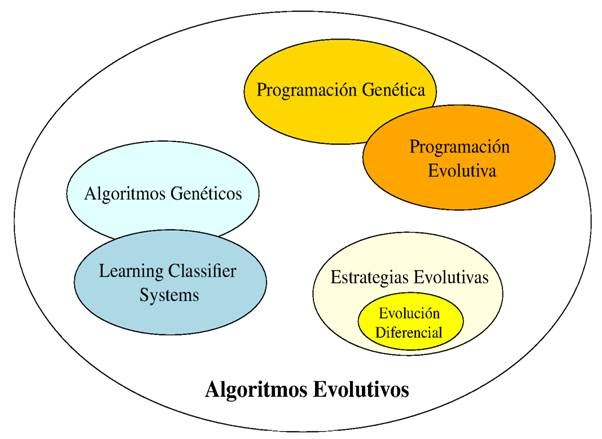
\includegraphics[width=12.8cm,height=8.1cm]{c21.jpg}
\caption{Esbozo gráfico de las distintas ramificaciones de los Algoritmos Evolutivos}
\end{figure}\break
Abordando un poco de contexto histórico éstas surgen en la década 
de 1950, sin embargo tuvieron su momento álgido hasta 1960 debido 
en gran medida a la creación de computadoras cada vez más potentes 
ya que como el lector podrá notar en secciones posteriores los 
recursos para llevar a cabo la ejecución de estos algoritmos no 
son pocos; por otra parte la concepción de dicho género pertenece 
a una rama más general denominada Cómputo Evolutivo en la cual 
han intervenido varios científicos para su forjamiento, sólo por 
mencionar algunos se tiene a Lawrence Jerome Fogel, John Henry 
Holland e Ingo Rechenberg, los cuales son los creadores de la 
Programación Evolutiva, Algoritmos Genéticos y las Estrategias 
Evolutivas respectivamente.\medskip\break
Cabe mencionar que la diferencia entre todas estas subdisciplinas 
radica en el hecho de que el proceso evolutivo aunque es esclarecedor 
también es genérico, motivo por el cual existen tantas ramificaciones 
de los Algoritmos Evolutivos como versiones de dicho procedimiento 
biológico y por ende de obtención de resultados.\medskip\break
Para fines del proyecto se considerarán únicamente a los Algoritmos 
Genéticos y las Estrategias Evolutivas debido a su implementación 
sencilla y abundancia de ejemplos, no obstante para proporcionar 
al lector de un panorama más amplio se muestra en la \hyperref[sec:c2_1]{\textcolor{blue}{Figura 2.1}} 
el diagrama con la mayoría de las técnicas que conforman a los 
Algoritmos Evolutivos.\medskip\break
Aún considerando el aspecto global del proceso evolutivo es 
posible precisar las etapas que determinan su comportamiento, 
de esta manera se toma una convención sobre las características 
mínimas que debe tener en cuenta una implementación en este 
rubro.\break
Tomando como base la \hyperref[sec:c2_2]{\textcolor{blue}{Figura 2.2}} 
se le presentan al lector no sólo las fases del procedimiento, 
sino también el orden en el que se llevan a cabo. A continuación 
se realiza una breve descripción:\medskip
\begin{figure}[ht]
%Se coloca el vínculo interno procedente del capítulo 2 (c2_2).
\label{sec:c2_2}
\centering
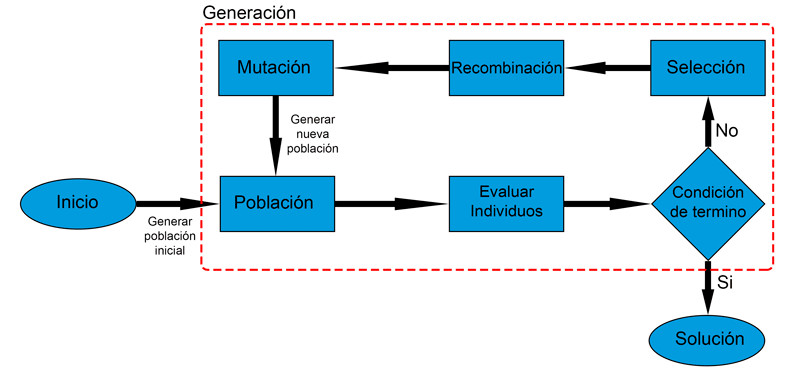
\includegraphics[width=13.5cm,height=7.9cm]{c22.png}
\caption{Fases del proceso evolutivo}
\end{figure}\break
En \textbf{Inicio} y \textbf{Población} la computadora ofrece 
un conjunto inicial de elementos aleatorios conocidos como 
\textit{individuos}, los cuales son los candidatos a la solución 
óptima, lo anterior indica que, debido a la naturaleza de su 
creación, existirán inicialmente individuos que no se acerquen 
tanto a la meta ideal como otros.\break
Como dato adicional, en algunas fuentes **(poner fuentes)** se 
utiliza el término \textit{cromosomas} para referirse de igual 
manera a dicho conjunto, sin embargo en este proyecto ambas 
palabras tendrán acepciones distintas.\medskip\break
La parte \textbf{Evaluar Individuos} implica la asignación de 
un valor escalar que determine la calidad de un individuo frente 
al problema que debe resolver. Para esto se apoya de un factor 
conocido como \hyperref[sec:c2_3]{\textbf{\textcolor{blue}{aptitud}}}.\medskip\break
La idea es entonces evolucionar a los individuos a través de 
técnicas que emulen la selección natural \hyperref[sec:c2_4]{\textbf{\textcolor{blue}{(Selección)}}}
y la generación de nuevos elementos \hyperref[sec:c2_5]{\textbf{\textcolor{blue}{(Recombinación ó Cruza}}}, \hyperref[sec:c2_6]{\textbf{\textcolor{blue}{Mutación)}}}) con la finalidad de obtener descendientes cada vez 
más aptos que, como se mencionó al principio, se acerquen más 
a la solución idónea.\break
Al proceso de creación de un nuevo conjunto de individuos se le 
conoce como \textit{generación}.\medskip\break 
Finalmente en el diagrama la porción correspondiente a \textbf{Condición de Término}
es meramente un requisito que indica que se ha alcanzado un 
límite para evitar que el proceso ecolutivo cicle indefinidamente, 
éste puede ser tanto un número límite de generaciones como un 
requisito alusivo a la aptitud.\medskip\break
Ahora utilizando la \hyperref[sec:c2_7]{\textcolor{blue}{Figura 2.3}} 
se expone de manera más sucinta la estructura interna de un 
individuo, así como algunos factores que giran en torno a 
éste:%\break
\begin{figure}[ht]
\centering
%Se coloca el vínculo interno procedente del capítulo 2 (c2_7).
\label{sec:c2_7}
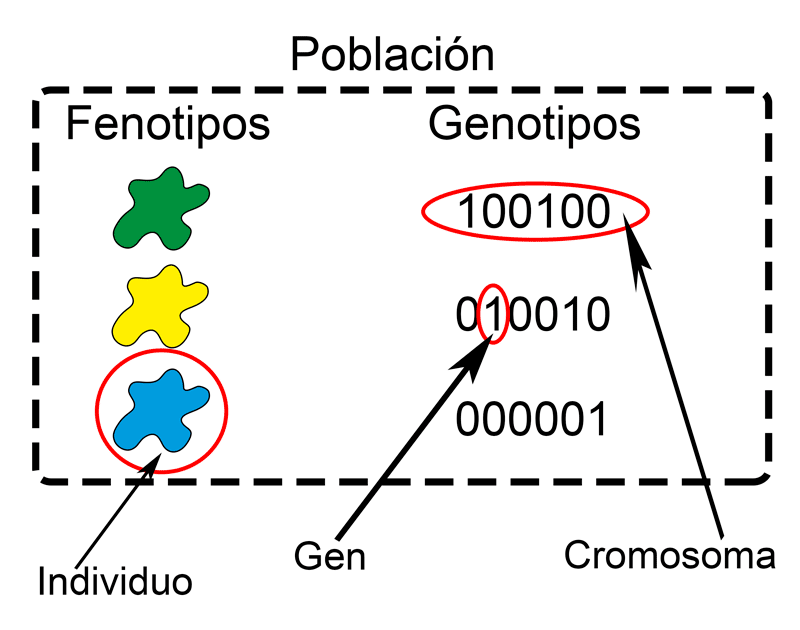
\includegraphics[width=13cm,height=8.1cm]{c23.png}
\caption{Elementos que conforman a un individuo}
\end{figure}\break
El primer término que el lector debe tomar en cuenta es el 
de \textit{población}; éste no es otra cosa que el conjunto 
de dos o más individuos.\break
Un concepto que no aparece aquí pero que será muy utilizado 
tanto en el el producto de software como en el Manual Técnico 
es el de \textit{comunidad}. De acuerdo a las bases biológicas 
\cite{b3} una comunidad es el conjunto de dos o más poblaciones 
y debido a la necesidad de operar con múltiples poblaciones 
simultáneamente en cada uno de los algoritmos se decidió crear 
una entidad con este nombre que no sólo satisfaciera las necesidades 
técnicas sino también que proporcionara un sentido biológico 
inherente al proyecto.\break
Como se aclaró previamente, se decidió mantener una escición
entre los conceptos \textit{cromosoma} e \textit{individuo} 
ya queen secciones posteriores será de gran utilidad puesto que, 
si bien en la práctica ambos conceptos se manejan indistintamente, 
esto ayudará a comprender mejor tanto el proceso evolutivo como 
sus implementaciones.\medskip\break
Entonces se define el cromosoma como una estructura que está 
conformada por elementos varios; tomando en cuenta que en el 
argot biológico ésta contiene proteínas, en el entorno computacional 
contendrá símbolos. Las definiciones que siguen corresponden 
a gen y alelo donde básicamente el primero es el espacio donde 
se puede almacenar los elementos antes mencionados respectivamente 
y a su vez el alelo es elemento en sí que va alojado en un gen.\medskip\break  
De lo anterior se incluyen dos conceptos clave que serán de utilidad 
genotipo y fenotipo: mientras que el genotipo se define prácticamente 
como una conjunción de genes (el cromosoma), el fenotipo es considerado 
como el resultado de haber procesado (expresado) el genotipo bajo un 
determinado entorno.

Luego, retomando el nivel de organización mayor conviene 
mencionar además algunos conceptos que van ligados a las 
interacciones entre las comunidades, entre los cuales se encuentran:

\begin{itemize}
\item Presión Selectiva - consiste en la implantación de algún 
tipo de catalizador en una población con la finalidad de obtener al 
mejor individuo generalmente bajo un número pequeño de generaciones. 
\item Especiación - se trata de un proceso en el cual, a partir de 
una población original se deriva al menos un descendiente, los cuales 
puedencompartir apenas pocas características en común. 
\item Epístasis - es considerada una situación en la interacción 
genética (genotipo) en la cual ***(poner referencia)*** una expresión 
de un gen (fenotipo) puede ser modificada radicalmente por la acción 
de dos o más de éstos. En términos más coloquiales la combinación de 
al menos dos genes puede dar un resultado totalmente diferente para 
el que se estaba pensado inicialmente. 
\end{itemize}

Una vez explicado todo el ámbito biológico sobre el cual se va a 
estar laborando, es momento de aterrizar todos estos conceptos 
y relaciones en una perspectiva computacional, se comienza entonces 
por describir de manera más sucinta todo lo relacionado con el 
cromosoma:

%Se inicia esta subsección dando paso a las funciones relacionadas
%con la representación cromosómica.
\subsection{Representación Cromosómica}
%Se coloca el vínculo interno procedente del capítulo 2 (c2_5).
\label{sec:c2_5}
Se define representación cromosómica a la forma de determinar 
el cromosoma y sus propiedades; como ya se mencionó previamente 
el cromosoma será portado por los individuos.\break
Aterrizando lo anterior en un entorno computacional el cromosoma 
consiste en una estructura de almacenamiento tipo arreglo donde cada 
uno de los espacios disponibles (genes) contendrán símbolos (alelos).
Para fines prácticos la representación tiene su base en dos variantes: 
binaria y punto flotante*** poner referencia
La primera sólo puede almacenar valores 1 y 0 en sus alelos mientras 
que la segunda puede almacenar cualquier valor que permita el equipo 
de cómputo en el que se esté implementando.

Una vez erigida la estructura computacional de un cromosoma y de
acuerdo al proceso evolutivo y como un paso intermedio, se debe
obtener el fenotipo, es decir, los resultados de haber procesado el 
genotipo, para ello se debe tomar la función de evaluación descrita al
comienzo y justamente a este paso previo se le denomina "evaluación de la
función objetivo.\break

Dicho lo anterior y con base en las evaluaciones de la función objetivo 
es necesario indicar una métrica que nos permita segmentar a los individuos 
del "peor" al "mejor", a ésta se le conoce como aptitud.

%A continuación se manejan en esta subsección las técnicas manejadas
%para la aptitud.
\subsection{Aptitud}
%Se coloca el vínculo interno procedente del capítulo 2 (c2_3).
\label{sec:c2_3}
Se denomina aptitud \footnote{También denominado \textit{aptitud}; 
durante el trabajo escrito ambos términos se usan indistintamente.} 
a un valor escalar que indica la calidad del individuo, esto es, 
a mayor aptitud, mayor es la probabilidad de que este sea la 
solución optima.\break
Indirectamente, esto nos indica que un individuo con un 
aptitud alto tiene más probabilidades de ser elegido y propagar 
su carga genética; así el criterio para escoger a un individuo 
está basado comúnmente en su aptitud.\medskip\break

De lo anterior se desprende que típicamente en las implementaciones
se asocia a un cromosoma con su aptitud, no obstante lo más adecuado
es ligar la aptitud con un individuo ya que, como se verá más 
adelante, es posible que de varios cromosomas inherentes a un individuo 
se obtenga un sólo resultado de aptitud 

Sólo como comentario adicional y con base en lo descrito en algunos 
párrafos previos, podemos aseverar que la aptitud se obtiene de los
fenotipos que se reciban de la evaluación en la función objetivo, 
por lo cual la gran mayoría de las opciones para asociar un cromosoma 
a una aptitud contienen características en común. 

Es importante mencionar que el listado de técnicas que se 
enuncian a continuación se muestran tal y como se han concebido 
originalmente, sin embargo para poder llevar a cabo el ajuste 
adecuado al ámbito Multiobjetivo es necesario reemplazar a la
función objetivo ($F_0$) por el Rankeo y a su vez alimentar éste 
por la evaluación de la función objetivo, del cual se hablará 
en el siguiente capítulo.\medskip\break

Los ejemplos mostrados para este proyecto son:

%Comienza la subsubsección dedicada a la aptitud Proporcional.
\subsubsection{Proporcional}
la aptitud está dado por la siguiente función:\medskip\break
\centerline{$Fitness(Individuo) = \frac{F_0(Individuo)}{\sum_{i=1}^{tama\tilde{n}o\_poblaci\acute{o}n}F_0(Individuo_i)}$}\medskip\break
Donde:

\begin{itemize}
\item $F_0$ es conocido como el valor de la función objetivo del 
individuo. Nótese que $F_0$ debe ser proporcional a la aptitud del 
individuo.
\end{itemize}

De acuerdo a la información provista anteriormente la asignación 
es llamada así porque, como dice el nombre, la aptitud de un 
individuo corresponde a la parte proporcional de la cantidad 
total de $F_0$ de la población.

%Empieza la subsubsección dedicada a la aptitud de Rankeo Lineal.
\subsubsection{Ranking Lineal}
Es denominado así porque la aptitud se asigna con una función 
lineal que tiene como fundamento la posición que ocupa el 
individuo dentro de la población.\break
El procedimiento es: los individuos se ordenan de acuerdo 
la evaluación en su función objetivo y entonces la aptitud 
se basa en la posición que cada uno de los individuos ocupa. 
Más en específico, la aptitud está proporcionado por la 
siguiente fórmula:\medskip\break
\centerline{$Fitness(Individuo) = 2 - SP + \frac{2 \cdot (SP - 1) \cdot posici\acute{o}n(Individuo)}{tama\tilde{n}o\_poblaci\acute{o}n - 1}$}\medskip\break
Donde:

\begin{itemize}
\item \textbf{SP (Selective Pressure ó Presión Selectiva)} es un valor que oscila entre 1 y 2.
\item \textbf{Posición(Individuo)} es la que ocupa el Individuo de acuerdo al rank.
\end{itemize}

Haciendo un análisis somero en la fórmula, se puede apreciar 
que los individuos con mejor aptitud serán aquéllos que se 
encuentren en las últimas posiciones.

%Inicia la subsubsección relativa a la aptitud de Rankeo 
%No Lineal.
\subsubsection{Rankeo No Lineal}
la aptitud se constituye ordenando los elementos de la 
población con base en su función objetivo y después 
tomando la posición del individuo y una función 
polinomial \textbf{(la cual es una función no lineal, de ahí el nombre)}. 
La fórmula es la siguiente:\medskip\break
\centerline{$Fitness(Individuo) = \frac{TP \cdot X^{posici\acute{o}n(Individuo)}}{\sum_{i=1}^{TP}X^{i - 1}}$}\medskip\break
Donde:

\begin{itemize}
\item \textbf{TP} es el tamaño de la Población.
\item \textbf{Posición(Individuo)} es la que ocupa éste de acuerdo al ranking previo.
\item \textbf{X} es la solución al polinomio: \((SP - TP) \cdot X^{TP - 1} + SP \cdot X^{TP - 2} + ... + SP \cdot X + SP = 0\)
\item \textbf{SP (Selective Pressure ó Presión Selectiva)} varía entre 1 y 2.
\end{itemize}

Realizando un análisis básico en la fórmula, al igual que 
con la aptitud anterior se puede apreciar que los individuos 
con mejor aptitud serán aquéllos que se encuentren en las 
últimas posiciones.

Una vez llevada a cabo la asignación de aptitud y de acuerdo
al esquema del proceso evolutivo, tiene lugar la operación de 
selección, la cual justamente obtiene típicamente  

%Se prosigue con la subsección que contiene el listado de técnicas 
%de selección.
\subsection{Selección}
%Se coloca el vínculo interno procedente del capítulo 2 (c2_4).
\label{sec:c2_4}
En la etapa de la selección la operación consiste en seleccionar 
los individuos en principio más aptos como resultado de 
la asignación de la opración anterior.
Durante dicha operación la importancia de la elección radica 
en la aptitud de cada individuo, además un individuo puede ser 
seleccionado más de una vez si la causa lo amerita.\break
De esta manera se elegirán tantos individuos como elementos haya 
en la población **agregar el reemplazo**.\medskip\break
El objetivo radica en mantener el equilibrio entre una ``selección 
justa'' y la oportunidad de permitir a los individuos con una 
calidad media o baja la propagación de su carga genética.\medskip\break
Cabe mencionar que en la mayoría de los casos se hará uso de un
valor denominado Valor Esperado \textbf{(ó Expected Value)}. 
El Valor Esperado para fines de este proyecto es el número de 
``hijos'' que un individuo puede ofrecer. Éste se calcula de 
la siguiente forma:\medskip\break
\centerline{$Valor\_Esperado(Individuo) = \frac{tama\tilde{n}o\_poblaci\acute{o}n \cdot Fitness(Individuo)}{\sum_{i=1}^{tama\tilde{n}o\_poblaci\acute{o}n}Fitness(Individuo_i)}$}\medskip\break
Entonces para este trabajo los tipos de selección desarrollados 
son:

%Comienza la subsubsección del método de selección llamado
%Ruleta
\subsubsection{Ruleta}
También es llamado Selección Proporcional.\break
En la función se distinguen dos etapas principales: construir 
la ruleta y ``ponerla a girar'' para que se elija al elemento.\break
Para la primera etapa se toma como base el Valor Esperado de 
cada individuo.\break
Al final aquéllos con Valores Esperados altos tendrán lugar 
a mayores espacios en la ruleta y por ende su probabilidad de 
elección aumenta.\medskip\break
Para recorrer la ruleta en realidad se toma un valor aleatorio 
entre 0 y la suma de los Valores Esperados; entonces se van 
sumando los Valores Esperados de los individuos hasta que se 
exceda el valor aleatorio mencionado antes.\break
Aquel elemento cuyo Valor Esperado haya excedido la suma se 
considera el elegido y es seleccionado para la etapa de cruza.\break
Esta segunda operación se efectúa tantas veces como el tamaño 
de la población.

%Tiene lugar el inicio de la subsubsección alusiva a la función
%de selección conocida como Torneo Probabilístico.
\subsubsection{Torneo Probabilístico}
Tal como lo sugiere el nombre, la selecciín será llevada a 
cabo en forma de competencia directa entre los individuos.\break
Tradicionalmente se comparan sus aptitud y de esta manera 
el individuo ganador es aquél con la cantidad mayor de aptitud, 
pero dado que se maneja un esquema probabilístico la 
decisión no depende totalmente del factor antes mencionado.\medskip\break
De esta manera se pueden recapitular los siguientes pasos:

\begin{enumerate}
\item Tomar $k\ (2 \leqslant k \leqslant tama\tilde{n}o\_poblaci\acute{o}n)$ individuos 
de la población.
\item Realizar el torneo de manera secuencial entre los 
elementos seleccionados anteriormente, esto es, tomar el 
elemento A y enfrentarlo con B, al resultado de la batalla 
anterior enfrentarlo con C y así sucesivamente.\break
Para ello por cada encuentro se crea un número aleatorio 
entre 0 y 1, si el número es menor a 0.5 se toma al elemento 
con menor aptitud, de lo contrario se elige al de mayor aptitud.\break
La operación se lleva a cabo hasta que se tenga un ganador 
de los $k$ individuos.
\item Los dos pasos anteriores se repiten hasta que se hayan 
obtenido tantos individuos como el tamaño de la población.
\end{enumerate}

%Ahora se muestra la subsubsección del método que lleva
%por nombre Muestreo Estocástico Universal.
\subsubsection{Muestreo Estocástico Universal}
El método consiste en lo siguiente:

\begin{enumerate}
\item Se selecciona un valor aleatorio entre 0 y 1, a éste se le 
llamará Pointer \textbf{(ó Puntero)}.
\item De manera secuencial se seleccionarán tantos individuos 
como el tamaño de la población, los cuales deben estar igualmente 
espaciados en su Valor Esperado tomando como referencia el valor 
de Pointer.
\end{enumerate}

Es importante aclarar el seguido punto, así que se abordará desde 
una perspectiva computacional:

\begin{itemize}
\item Se deben tener variables adicionales que indiquen la 
acumulación tanto del Pointer \textbf{(CP, Cumulative Pointers)} 
como de los Valores Esperados \textbf{(CEV, Cumulative Expected Value)} 
así como al individuo actual que está siendo seleccionado \textbf{(I)}.
\item Para averiguar si un individuo está igualmente espaciado en 
su Valor Esperado con respecto de los demás basándose en Pointer, 
basta con corroborar que:\medskip\break
\centerline{$CP + Pointer > CEV + EV$}\medskip\break
Si la condición descrita es verdadera los valores EV e I deben 
actualizarse \textbf{(I se ajusta al siguiente individuo)} ya 
que esto indica que se buscará al siguiente individuo espaciado 
equitativamente con el valor Pointer. No se hace nada si la 
condición es falsa.
\item Independientemente del valor de la condición anterior, CP 
y CEV deben actualizarse durante todo el ciclo.
\end{itemize}
Cabe mencionar que si la lista de individuos se agota, se puede 
volver a iterar desde el inicio teniendo cautela en conservar CEV 
y CP.




%Ahora en esta subsección se realiza el desglose de las técnicas 
%de cruza.
\subsection{Cruza}
%Se coloca el vínculo interno procedente del capítulo 2 (c2_5).
\label{sec:c2_5}
Prosiguiendo con el ciclo de creación de una nueva población, 
es en este apartado donde se lleva a cabo la concepción de nuevos 
individuos.\break
Debido a esto se busca crear ``hijos'' más aptos que respondan 
mejor ante la problemática fundamentada, es decir, concebir 
soluciones que se adapten mejor a los criterios establecidos 
por el usuario desde un inicio basándose en las soluciones 
predecesoras.\break
Es menester mencionar que esta función es meramente binaria, 
lo cual significa que siempre deben haber dos padres y siempre 
debe regresar dos hijos.\medskip\break
Las implementaciones desarrolladas son:

%Comienza la subsubsección de la función de cruza conocida como
%N Puntos.
\subsubsection{N-Puntos}
Su funcionamiento consiste en construir a los descendientes 
usando sub-bloques de cromosomas de cada uno de los padres, 
determinados éstos por una cierta cantidad de puntos de corte, 
de ahí el nombre. Aterrizando lo anterior de una manera concisa 
se tiene lo siguiente:\medskip\break
Consideremos a los cromosomas de los padres Padre I: 
$I_1I_2...I_n$ y Padre J: $J_1J_2...J_n$.\break
Posteriormente se determinan aleatoriamente los puntos de corte, 
cabe mencionar que si los cromosomas son de tamaño $n$, pueden 
existir máximo $n - 1$ puntos. Supongamos que se crean $k$ puntos 
$(1 \leqslant k \leqslant n - 1)$ y por lo tanto cada cromosoma 
queda separado en $k + 1$ bloques.\break
De esta manera obtenemos:

\begin{itemize}
\item Padre I en bloques \textbf{(BI)}: $BI_1BI_2...BI_{k + 1}$;
\item Padre J en bloques \textbf{(BJ)}: $BJ_1BJ_2...BJ_{k + 1}$.
\end{itemize}

Finalmente cada hijo constará de la alternancia de bloques de 
manera secuencial comenzando por el bloque inicial de un padre 
determinado, dicho de otra forma, los hijos estarán constituidos 
de la siguiente manera:

\begin{itemize}
\item Para el hijo $H_1$: $BI_1BJ_2...BI_{k + 1}$
\item Para el hijo $H_2$: $BJ_1BI_2...BJ_{k + 1}$
\end{itemize}

%A continuación se muestra la subsubsección de la técnica de cruza
%denominada Uniforme.
\subsubsection{Uniforme}
La característica de este procedimiento es la de crear nuevos 
individuos intercambiando secuencialmente los genes de sus 
padres; visto de una manera más estructurada consiste en 
lo siguiente:\medskip\break
Tenemos a los cromosomas de los padres Padre A: $A_1A_2...A_n$ 
y Padre B: $B_1B_2...B_n$.\break
Ahora, cada hijo será construido con genes de uno y sólo uno 
de los padres a menos que se indique lo contrario; este 
movimiento será posible con una variable denominada Pmask 
\textbf{(Pm)} que toma valores de 0 a 1 y una probabilidad 
de Pmask \textbf{(Pp)} que también toma valores de 0 a 1. 
Entonces lo anterior se puede declarar así:\medskip\break
Para el hijo $(H_1)$ que tomará sus genes del padre A \textbf{(PA)}:

\begin{itemize}
\item Si $Pm \leqslant Pp\ entonces\ H_1(i) = A_i,\ en\ otro\ caso\ H_1(i) = B_i; 1 \leqslant i \leqslant n$.
\end{itemize}
Para el hijo \((H_2)\) que tomará sus genes del padre B \textbf{(PB)}:
\begin{itemize}
\item Si $Pm \leqslant Pp\ entonces\ H_2(i) = B_i,\ en\ otro\ caso\ H_1(i) = A_i; 1 \leqslant i \leqslant n$.
\end{itemize}

%A continuación comienza la subsección relacionada con las 
%funciones de mutación.
\subsection{Mutación}
%Se coloca el vínculo interno procedente del capítulo 2 (c2_6).
\label{sec:c2_6}
Retomando el proceso de creación de una nueva población, es 
aquí donde una vez obtenidos los hijos, se modifican los alelos 
de sus cromosomas de manera individual.\break
Con esto se persigue principalmente que estas ínfimas alteraciones 
permitan incrementar la exploración del material genético y por 
ende otorgar individuos aún más aptos sin caer en el peligro de 
perder características valiosas en la población.\break
Considerando lo anterior, lo primero que hay que tomar en cuenta 
es que la operación de mutación es unaria, esto significa que 
sólo se puede mutar el cromosoma de un individuo a la vez.\medskip\break
Para este trabajo las implementaciones son las siguientes:

%Principia la subsubsección de la técnica de mutación Binaria.
\subsubsection{Binaria}
El procedimiento es el siguiente:

\begin{enumerate}
\item Se trata cada gen individualmente y se modifica su 
alelo correspondiente de acuerdo a una probabilidad de mutación 
asignada, si ésta es suficiente se procede a hacer el cambio, 
en otro caso se deja el alelo asociado al gen intacto.
\item Retomando el caso en que se puede modificar el alelo 
del gen se verifica su valor actual y ya que se maneja una 
representación binaria su transformación es muy simple: si 
se encuentra un 0, el alelo toma el valor 1 y viceversa.
\end{enumerate}

%Comienza la subsubsección del método de mutación de Punto
%Flotante.
\subsubsection{Punto Flotante}
El procedimiento es el siguiente:

\begin{enumerate}
\item Se verifica cada gen individualmente y se altera su 
alelo pertinente de acuerdo a una probabilidad de mutación 
asignada, si ésta es suficiente se procede a hacer el cambio, 
en otro caso se deja el alelo asociado al gen intacto.
\item Retomando el caso en que se puede modificar el alelo 
del gen se verifica los límites de la variable de decisión 
que está ligada a éste, así como la precisión decimal. 
Entonces se crea el nuevo número con la precisión decimal 
requerida y se sustituye por el anterior.
\end{enumerate}


Paso del elitismo en teoría sólo se agregan las poblaciones m + L etc para este tema y pos fines de simplicidad
blabla blabla

%A continuación se lleva a cabo el desarrollo de la sección
%relativo a la Optimización Multiobjetivo.
\section{Optimización Multiobjetivo}
En un lenguaje coloquial, la Optimización Multiobjetivo consiste 
en, dado un listado de objetivos, encontrar la solución que 
optimice el rendimiento de cada uno de éstos bajo un cierto 
conjunto de restricciones. Las condiciones de búsqueda son 
variadas, pero por lo general los objetivos tendrán conflictos 
entre sí, lo que quiere decir que el hecho de hallar una solución 
excelente para un objetivo puede significar la paupérrima para 
otro, por ello es que se debe ser cauteloso en la adquisición 
de soluciones.\medskip\break
Lo anterior aterrizado en un lenguaje matemático consiste en lo 
siguiente:
Tenemos un vector de funciones objetivo:\medskip\break
\centerline{$F(\vec{x}) = [f_1(\vec{x}),f_2(\vec{x}),...,f_n(\vec{x})]^T; con\ n \geqslant 1.$}\medskip\break
Donde:\medskip\break
\centerline{$\vec{x} = [x_1,x_2,...,x_k]^T;\ k \geqslant 1.$}\medskip\break
Representa al vector de variables de decisión que cada función 
objetivo recibe como parámetro.
La meta es encontrar un vector especial de variables de decisión 
denominado:\medskip\break
\centerline{$\vec{x}^{*} = [x_1^{*},x_2^{*},...,x_k^{*}]^T;\ k \geqslant 1.$}
Tal que:\medskip\break
\centerline{$f_i(\vec{x}^{*}) \leqslant f_i(\vec{x});\ 1 \leqslant i \leqslant n;\ \forall f \in F$}.\medskip\break
Dicho de otra forma, se debe encontrar el vector de variables de 
decisión que minimize todas y cada una de las funciones objetivo 
en existencia.
Adicionalmente, todo vector de variables de decisión debe estar 
sujeto a las restricciones:\medskip\break
\centerline{$h_i(\vec{x}) = 0;\ 1 \leqslant i \leqslant p\ \ (restricciones\ de\ igualdad).$}
\centerline{$g_i(\vec{x}) \leqslant 0;\ 1 \leqslant i \leqslant m\ \ (restricciones\ de\ desigualdad).$}\medskip\break
Las cuales para fines de este proyecto son aquéllas a las que 
se encuentran afianzadas las variables de decisión.\medskip\break
Algo importante a mencionar es que en las definiciones se trata 
únicamente la minimización de funciones objetivo porque, en caso 
de solicitar la maximización, simplemente se realiza la sustitución:\medskip\break
\centerline{$f'_i(\vec{x}) = -f_i(\vec{x});\ 1 \leqslant i \leqslant n,\ para\ alguna\ f \in F.$}\medskip\break
Es decir, minimizando la función negativa se obtiene el máximo. 
El producto de software ya contempla este tipo de casos.\medskip\break
También es preciso añadir la diferencia entre los términos 
Multiobjetivo y Multicriterio; mientras que el primero contempla 
a más de una función objetivo, el segundo hace lo propio con 
respecto de las variables de decisión, por ello es que en un 
problema de optimización pueden encontrarse ambos escenarios; 
si bien en este trabajo de tesis se le da prioridad a la faceta 
Multiobjetivo en pruebas ulteriores se tratará con ejemplos 
considerados Multicriterio también.

%A continuación se explica el concepto denominado Optimalidad 
%de Pareto, el cual se utiliza en la Optimización Multiobjetivo.
\subsection{Optimalidad de Pareto}      
Como se ha podido apreciar hasta este punto la Optimización 
Multiobjetivo prácticamente se sustenta en comparaciones y 
operaciones entre vectores; de lo anterior se deriva la 
necesidad de establecer un criterio para determinar la superioridad 
de un vector frente a otro y así otorgar la solución idónea.\break
Si bien existen considerables maneras de lograr este objetivo, 
para fines del proyecto presentado se toma en cuenta aquélla 
conocida como la \textbf{Eficiencia u Optimalidad de Pareto}.\medskip\break
Haciendo alusión al contexto histórico este concepto fue 
creado por el economista italiano Vilfredo Pareto, quien basado 
en los trabajos de Edgeworth \cite{b4} concibió en 1896 una 
propuesta de equilibrio en el cual se beneficia a un elemento 
sin perjudicar a otro y viceversa, así cuando esta situación 
se torna insostenible entonces el equilibrio pierde sentido.\break
Concretando el enunciado previo con base en definiciones la 
primera que se utiliza es la de \textbf{Dominancia de Pareto} ó 
simplemente dominancia entre vectores, para ello se toman los 
vectores $U = (u_1 , u_2 , ..., u_k)$ y $V = (v_1 , v_2 , ..., v_k)$ 
y se dice que \textit{U domina a V} ó \textit{V es dominada por U si}:\medskip\break
\centerline{$\forall i\ u_i \leq v_i \land \exists i\ u_i < v_i;\ i \in \{1, ..., k\}$.}\medskip\break
Esto significa que $U$ debe ser menor que $V$ en cada uno de sus 
componentes para garantizar la dominancia.
La simbología que se suele usar para identificar este hecho es $u \succ v$.\medskip\break
Conviene mencionar la existencia de dos tipos de dominancias: 
fuerte y débil; la primera es prácticamente la definición 
construida para la comparación entre vectores, mientras que 
la segunda únicamente prescinde de la condición de existencia 
menor estricta.\break
Esto sólo se menciona con fines ilustrativos ya que a pesar de 
dicha distinción únicamente se trabajará con la dominancia fuerte, 
si bien computacionalmente toma más tiempo calcularla, es más 
precisa y por ende se arrojan resultados más concisos que usando 
la contraparte débil.\medskip\break
Tomando el enunciado previo sobre dominancia y aquéllos creados en 
la sección de Optimización Multiobjetivo, se introducen los conceptos 
\textbf{Óptimo de Pareto} y \textbf{Frente de Pareto}.\break
El primero, también denominado \textbf{Conjunto Optimo de Pareto} 
($P^{*}$ o $P_{true}$) es aquél que cumple con la siguiente condición:\medskip\break
\centerline{$P^{*} := \{ \vec{x}\ |\ \vec{F}(\vec{x}) \succ \vec{F}(\vec{x}');\ \forall \vec{x}' \in FS \}$.}\medskip\break
Nótese que de hecho el Conjunto Óptimo de Pareto es equivalente 
a la obtención de todos los vectores $\vec{x}^{*}$ de la sección de 
Optimización Multiobjetivo, además FS es conocido como la región 
factible o lo que es lo mismo el espacio plausible de todas las 
variables de decisión; como consecuencia se tiene que $P^{*} \subseteq FS \subseteq IR^{n}$.\medskip\break
Ahora el Frente de Pareto es el conjunto descrito a continuación:\medskip\break
\centerline{$PF^{*} := \{ \vec{z}^{*} = \vec{F}^{*}(\vec{x}^{*}) = [f_1^{*}(\vec{x}^{*}),\ f_2^{*}(\vec{x}^{*}), ...,\ f_n^{*}(\vec{x}^{*})]\ |\ \vec{x}^{*} \in P^{*} \}$.}\medskip\break
El cual no es otra cosa que la recopilación de las evaluaciones 
del Óptimo de Pareto en las funciones objetivo.\break
Dicho de otra forma, el Óptimo de Pareto corresponde al conjunto 
de las soluciones en el espacio de variables de decisión, mientras 
que el Frente de Pareto es lo análogo con respecto del espacio de 
funciones objetivo.\medskip\break
Generalizando, al final un problema de Optimización Multiobjetivo 
se reduce en encontrar el Frente de Pareto, no obstante de acuerdo 
con el Dr. Coello \cite{b5} no existe una forma analítica de obtener 
el Óptimo de Pareto \textbf{(y por ende el Frente de Pareto)}, lo 
que significa que se deben utilizar aproximaciones para encontrar 
el resultado deseado.\break
Es aquí donde entra el uso de los Algoritmos Evolutivos descritos en 
la sección anterior, destacando además que esta es sólo una de las 
numerosas aproximaciones elaboradas \cite{b6} para encontrar el ya 
mencionado Frente de Pareto.\break
Debido al alcance de este proyecto, tales técnicas alternativas no 
se mencionan.

%https://www.google.com.mx/search?q=multi+objective+evolutionary+algorithm+diagram&tbm=isch&source=iu&ictx=1&fir=868gdaZPoA3UmM%253A%252CqDoaNIynX99gdM%252C_&usg=AI4_-kQU3NfAVyhXZ4wmURV9yVuMxg3syg&sa=X&ved=2ahUKEwi61Jj8_bHeAhUNG6wKHWNRAV0Q9QEwA3oECAUQCg#imgrc=ax98ZCp-sQ-NCM:

agregar las definiciones.

%Termina el documento.
\end{document}


       %Ahora se coloca la información que se encuentra en el archivo chapter3.tex.
       %Autor: Aarón Martín Castillo Medina.
%Asesora: Dra. Katya Rodríguez Vázquez
%Contacto: katya.rodriguez@iimas.unam.mx; amcm329@hotmail.com

%Este archivo contiene información relacionada con las características,
%algoritmos y aplicaciones relacionados con los M.O.E.A.'s así como las 
%métricas de desempeño que se utilizarán e incluso una introducción al
%producto de software elaborado con base en todo lo anterior.


%Se indica que el documento es de tipo reporte bajo el paquete standalone.
\documentclass[class=report, crop=false]{standalone}

%Se añaden los paquetes a usarse localizados en packages_used_standard.sty
\usepackage{packages_used_standard}

%Comienza el documento.
\begin{document}

%Comienza el capítulo relacionado con la estructura interna,
%ejemplos y métricas alusivas a un M.O.E.A.
\chapter {M.O.E.A.}

%%%%%%%%%%%%%%%%%%%%%%%%%%%%%%%%%%%%%%%%%%%%%%%%%%%%%%%%%%%%%%

\section{Rankeo}

\section{Aptitud Compartida}  
También llamado Shared Fitness

\section{Algoritmos}
Con base en el capítulo anterior, el funcionamiento de un M.O.E.A. 
\textbf{(resolver un problema de optimización multiobjetivo usando 
algoritmos evolutivos)} generalmente se lleva a cabo de la siguiente 
manera:

\begin{enumerate}[1.]
\item Usando una Representación Cromosómica, crear la Población Padre y evaluar cada uno de los Individuos respecto a las funciones objetivo.

\item Asignar un Ranking a los Individuos de la Población Padre.  

\item Con base en el Ranking, asignar la Aptitud \textbf{(en inglés Fitness)} a cada uno de los Individuos.

\item Tomando en cuenta el Fitness, aplicar las operaciones de Selección, Cruza y Mutación con la finalidad de crear una Población Hija. Todos los métodos empleados en este punto deben funcionar acorde a la Representación Cromosómica del punto 1.

\item \textbf{(Opcional)} Utilizar el Fitness Compartido \textbf{(en inglés Shared Fitness)} para aplicar una elección más minuciosa de los mejores Individuos en la Población Hija. 

\item Designar a la población Hija como la nueva población Padre.

\item Repetir los pasos 2 a 6 hasta haber alcanzado un número límite de generaciones \textbf{(iteraciones)}. 
\end{enumerate}

A grandes rasgos la diferencia entre un M.O.E.A. y otro es la Presión Selectiva 
\textbf{(en inglés Selective Pressure)} que se aplica durante el procedimiento, para fines de este proyecto
se trata de la tolerancia para seleccionar a los Individuos de calidad media o baja frente a los
mejores. Una baja Presión Selectiva permite elegir Individuos no tan aptos; el caso es análogo para
una alta Presión Selectiva.



\subsection{V.E.G.A.}
La forma de proceder del algoritmo es la siguiente:

\begin{enumerate} 
\item Se crea la Población Padre (de tamaño \(n\)).
\item Tomando en cuenta las \(k\) funciones objetivo y la Población Padre, se crean \(k\) subpoblaciones de tamaño \(n/k\) cada una, si este número llega a ser irracional se pueden hacer ajustes con respecto de la distribución de los Individuos.
\item Por cada subpoblación, se aplica la técnica de Selección y obtienen los \(n/k\) Individuos, terminado esto se deben unificar todos los seleccionados de nuevo en una súper Población.
\item Con la súper Población del paso 3, se crea a la población Hija, la cual pasará a convertirse en la la nueva Población Padre.
\item Se repiten los pasos 2 a 4 hasta haber alcanzado el número de generaciones \textbf{(iteraciones)} límite.
\end{enumerate}

Como se puede apreciar es una implementación muy sencilla 
de optimización multiobjetivo, sin embargo el inconveniente 
que tiene es la fácil pérdida de material genético valioso.\break
Lo anterior significa que un Individuo que en una generación 
previa era el mejor para una función objetivo \(i\) al momento 
de ser separado y seleccionado en una subpoblación \(j\) \textbf{(y por ende analizado bajo la función objetivo \(j\))} 
puede ser muy malo en calidad y por tanto no ser seleccionado;
perdiéndose la ganancia genética hasta el momento obtenida para 
la función objetivo \(i;\ i \neq j\).\medskip\break
Por ello es que se puede decir que V.E.G.A. genera soluciones 
promedio que destacan con una calidad media para todas las 
funciones objetivo.\medskip\break
Finalmente hay que comentar que para este algoritmo no se requiere 
aplicar un Ranking específico, no obstante, se ha decidido utilizar 
el de Fonseca \& Flemming \textbf{(véase Model/Community/Community.py)} 
pues es el más sencillo de implementar.

\subsection{M.O.G.A.}
Su funcionamiento es el siguiente:

\begin{enumerate} 
\item Se crea la Población Padre, se evalúan las funciones objetivo de sus correspondientes Individuos.
\item Se asigna a los Individuos un Ranking \textbf{(Fonseca \& Flemming)} y posteriormente se calcula el Niche Count de la Población Padre.
\item Tomando en cuenta los valores del punto 2 se obtiene el Fitness para cada Individuo y posteriormente su Shared Fitness.
\item Se aplica el operador de selección sobre la Población Padre para determinar los elegidos para dejar descendencia.
\item Se crea la Población Hija, se evalúan las funciones objetivo de sus correspondientes Individuos.
\item Se asigna a los Individuos un Ranking \textbf{(Fonseca \& Flemming)} y posteriormente se calcula el Niche Count de la Población Hija.
\item Tomando en cuenta los valores del punto 6 se obtiene el Fitness para cada Individuo y posteriormente su Shared Fitness.
\item La Población Hija pasará a ser la nueva Población Padre.
\item Se repiten los pasos 4 a 8 hasta que se haya alcanzado el número límite de generaciones \textbf{(iteraciones)}.
\end{enumerate}

Como se puede apreciar, la implementación de este algoritmo es 
muy sencilla, además se rige casi en su totalidad por el 
Shared Fitness \textbf{(ó Fitness Compartido)}, por lo que 
la Presión Selectiva \textbf{(ó Selective Pressure)} incluida 
dependerá en gran medida de la función de Distancia que se utilice, 
así como de la magnitud indicada por el usuario.\medskip\break
Finalmente es menester mencionar que para esta implementación el 
Ranking utilizado debe ser estrictamente el de Fonseca \& Flemming 

\subsection{S.P.E.A. 2}
Se desarrolla la implementación de la técnica M.O.E.A. 
conocida como S.P.E.A. II \textbf{(Strength Pareto Evolutionary Algorithm ó Algoritmo Evolutivo de Fuerza de Pareto)}.\break
El funcionamiento del algoritmo es el siguiente:

\begin{enumerate}
\item Se inicializa una población llamada \emph{P} y un conjunto inicialmente vacío llamado \emph{E} \textbf{(E albergará Individuos también)}; ambos son de tamaño n.
\item Se asigna el Fitness a los Individuos de \emph{P} y \emph{E} \textbf{(para ello se evalúan las funciones objetivo de los Individuos de ambos conjuntos y se asigna el Ranking Zitzler \& Thiele)}.
\item A continuación se funden \emph{P} y \emph{E} en una súper Población \textbf{(llamémosle S también señalado en el algoritmo como Mating Pool, de tamaño n)}.Para ello primero se añaden los Individuos \emph{NO DOMINADOS} de \emph{P} en \emph{S} y posteriormente los \emph{NO DOMINADOS} de \emph{E} en \emph{S}.\break 
Aquí se distinguen dos casos:
      \begin{itemize}
      \item Si llegasen a faltar Individuos se añaden al azar Individuos \emph{DOMINADOS} de \emph{P} en \emph{S} hasta completar la demanda.
      \item Si después de la fusión el número de Individuos supera a n, entonces se hace un truncamiento en \emph{S} hasta ajustar su tamaño a n.
      \end{itemize}
\item \emph{S} será la nueva \emph{E}, además se crea la población Hija de la recién creada \emph{E} \textbf{(E-Child)}.
\item E-Child será la nueva P.
\item Se repiten los pasos 2 a 5 hasta que se haya alcanzado el límite de generaciones \textbf{(iteraciones)}.
\end{enumerate}

Finalmente lo que se regresa es \emph{E}, ya que ahí es 
donde se han almacenado los mejores Individuos de todas 
las generaciones.\medskip\break
La característica de este algoritmo es que tiene una 
Presión Selectiva alta ya que se da prioridad a los 
Individuos no dominados \textbf{(de ahí el nombre de Fuerza de Pareto ó los más fuertes con respecto al principio de Pareto)},
y el hecho de mezclar a \emph{E} y \emph{P} en una 
súper Población garantiza la conservación de los mejores 
Individuos sin importar el transcurso de las generaciones \textbf{(a eso se le conoce como Elitismo)}, 
pero también da una tolerancia, aunque mínima, a los Individuos 
de menor calidad como en el punto 3.\break
Además al momento de actualizar \emph{S} a \emph{E} y 
E-Child a \emph{P} se tiene una especie de seguro de vida, 
es decir, si en algún momento la población E-Child llegara a
tener una calidad baja se tiene el respaldo de \emph{E} 
para una generación posterior para formar \emph{S}.\medskip\break
Se debe tener en cuenta que el algoritmo originalmente no 
contempla ni una súper Población \emph{S} ni E-Child 
sino que en los pasos 3 y 4 se utiliza solamente \emph{E} 
para referirse tanto a E-child como a \emph{S}, sin embargo 
para no confundir al usuario en la funcionalidad del método 
se decidió colocar contenedores extra para poder diferenciar 
más precisamente a los elementos involucrados.\medskip\break
Algo muy importante a mencionar es que en el paso 1 y al momento 
de crear la población E-Child es necesario evaluar las funciones 
objetivo, asignar un Ranking y posteriormente un Fitness para 
que se puedan aplicar los operadores geneticos \textbf{(véase Model/GeneticOperator)}, 
para este caso el Ranking es estrictamente el de Zitzler \& Thiele; 

\subsection{N.S.G.A. II}
La forma de proceder del método es la siguiente:

\begin{enumerate}
\item Se crea una Población Padre \textbf{(de tamaño n)}, a la cual se le evalúan las funciones objetivo de sus Individuos, se les asigna un Ranking \textbf{(Goldberg)} y posteriormente se les otorga un Fitness.
\item Con base en la Población Padre se aplica el operador de Selección para elegir a los Individuos que serán aptos para reproducirse.
\item Usando a los elementos del punto 2, se crea una Población Hija \textbf{(de tamaño n)}.
\item Se crea una súper Población \textbf{(llamémosle S, de tamaño 2n)} que albergará todos los Individuos tanto de la Población Padre como Hija; a \emph{S} se le evalúan las funciones objetivo de sus Individuos, se les asigna un Ranking \textbf{(Goldberg)} y posteriormente se les otorga un Fitness.
\item La súper Población \emph{S} se divide en subcategorías de acuerdo a los niveles de dominancia que existan, es decir, existirá la categoría de dominancia 0, la cual almacena Individuos que tengan una dominancia de 0 Individuos \textbf{(ningún Individuo los domina)}, existirá la categoría de dominancia 1 con el significado análogo y así sucesivamente hasta haber cubierto todos los niveles de dominancia existentes.
\item Se construye la nueva Población Padre, pare ello constará de los Individuos de \emph{S} donde la prioridad será el nivel de dominancia, es decir, primero se añaden los elementos del nivel 0,luego los del nivel 1 y así en lo sucesivo hasta haber adquirido n elementos.
Se debe aclarar que la adquisición de Individuos por nivel debe ser total, esto significa que no se pueden dejar Individuos sueltos para el mismo nivel de dominancia.\break
Supongamos que a un nivel k existen tantos Individuos que su presunta adquisición supera el tamaño n, en este caso se debe hacer lo siguiente:
      \begin{enumerate}
      \item Se crea una Población provisional \textbf{(Prov)} con los Individuos del nivel k, se evalúan las funciones objetivo a cada uno de sus Individuos, se les asigna un Ranking \textbf{(Goldberg)} y posteriormente se les asigna el Fitness.\break
            Con los valores anteriores se calcula el Niche Count \textbf{(véase Model/SharingFunction)} de los Individuos; una vez hecho ésto se seleccionan desde Prov los Individuos faltantes con los mayores Niche Count, esto hasta completar el tamaño n de la nueva Población Padre.
      \end{enumerate}
\item Al haber conformado la nueva Población Padre, se evalúan las funciones objetivo de sus Individuos, se les asigna el Ranking correspondiente \textbf{(Goldberg)} y se les atribuye su Fitness.
\item Se repiten los pasos 2 a 7 hasta haber alcanzado el límite de generaciones \textbf{(iteraciones)}.
\end{enumerate}

Como su nombre lo indica, la característica de este algoritmo es 
la clasificación de los Individuos en niveles para su posterior 
selección.\break
Esto al principio propicia una Presión Selectiva moderada por 
la ausencia de elementos con dominancia baja que suele existir 
en las primeras generaciones, sin embargo en iteraciones posteriores 
se agudiza la Presión Selectiva ya que eventualmente la mayoría de 
los Individuos serán alojados en las primeras categorías de dominancia, 
cubriendo casi instantáneamente la demanda de Individuos necesaria en 
el paso 6, por lo que las categorías posteriores serán cada vez 
menos necesarias con el paso de los ciclos.\medskip\break
Por otra parte la fusión de las Poblaciones en \emph{S} garantiza 
que siempre se conserven a los mejores Individuos independientemente 
de la generación transcurrida, a eso se le llama Elitismo.\break
Por cierto que en el algoritmo original no existe un nombre oficial 
para \emph{S} sino más bien se señala como una estructura genérica, 
sin embargo se le ha formalizado con un identificador para guiar 
apropiadamente al usuario en el flujo del algoritmo.\medskip\break
Para finalizar se señala que el uso del ranking de Goldberg 

\section{M.O.P.}      
\section{Indicadores de Desempeño}
\section{Introducción a M.O.E.A Software}
Habiendo detallado todos los elementos 

M.O.E.A. Software surge como una solución ante la problemática blablabla.

Para abordar detalles de índole más técnica se recomienda visitar la sección **Características Técnicas** perteneciente al Apéndice.

\label{sec:p_1}    

%Termina el documento.
\end{document}

       
       %Luego se inserta la información del archivo chapter4.tex.
       %Autor: Aarón Martín Castillo Medina.
%Asesora: Dra. Katya Rodríguez Vázquez
%Contacto: katya.rodriguez@iimas.unam.mx; amcm329@hotmail.com

%Este archivo contiene las pruebas hechas con el producto de software
%abordado en el capítulo anterior, además de la comparación entre éstos
%usando las métricas consideradas en el mismo capítulo mencionado.


%Se indica que el documento es de tipo reporte bajo el paquete standalone.
\documentclass[class=report, crop=false]{standalone}

%Se añaden los paquetes a usarse localizados en packages_used_standard.sty
\usepackage{packages_used_standard}

%Comienza el documento.
\begin{document}

%Comienza el capítulo relacionado con la Experimentación y
%Análisis de Resultados.
\chapter{Experimentación y Análisis de Resultados}

Decir de los elementos para llegar a los \cite{b7} resultados.

%Termina el documento.
\end{document}


       %Luego se inserta la información del archivo chapter5.tex.
       %Autor: Aarón Martín Castillo Medina.
%Asesora: Dra. Katya Rodríguez Vázquez
%Contacto: katya.rodriguez@iimas.unam.mx; amcm329@hotmail.com

%Este archivo almacena las conclusiones obtenidas a partir de las
%pruebas elaboradas en el capítulo previo; también se hace mención
%de las posibilidades de expansión y enriquecimiento del trabajo para
%el futuro.


%Se indica que el documento es de tipo reporte bajo el paquete standalone. 
\documentclass[class=report, crop=false]{standalone}

%Se cargan todos los paquetes que residen en el archivo packages_used_standard.sty
\usepackage{packages_used_standard}

%Empieza el documento.
\begin{document}

\chapter{Conclusiones}
Con base en los resultados anteriores se puede 
primeramente verificar que

\section{Trabajo Futuro}
Una vez que se han concretado los méritos y metas cumplidas del 
presente trabajo escrito conviene mencionar los posibles escenarios 
de expansión del proyecto, ante lo cual se pueden dividir en dos 
categorías: analítica y técnica.

En lo concerniente a la primera

Ahora en consideración a la segunda el tratamiento se enfoca 
principalmente en las características relacionadas con M.O.E.A. 
Software.

En primer lugar, debido a la carencia de tiempo y limitaciones 
tecnológicas, las restricciones que están sujetas a las 
variables de decisión hasta el cierre de este trabajo corresponden 
unicamente a valores escalares aún teniendo en cuenta que las 
definiciones vistasen un principio contemplan el uso de funciones. 
Por este motivo se debe tener en mente la inclusión de esta 
caracterítica para futuras versiones del programa.

Se manifiesta un escenario parecido con las funciones objetivo 
ya que el producto de software no considera aquéllas definidas a 
trozos que, aunque no forman parte de la versión actual, son 
imprescindibles puesto que muchos de los M.O.P.’s adicionales 
localizados en las fuentes de consulta****** contienen funciones 
de este tipo.
Desde una perspectiva gráfica, la interfaz elaborada hasta el 
momento resulta insuficiente debido a que durante el proceso se 
hallaron varias fallas originadas en el uso de bibliotecas que 
carecían de mantenimiento, no obstante se utilizaron debido a su 
portabilidad con todos los sistemas operativos.
Es por esta razón que se puede sugerir el uso de alguna otra 
tecnología gráfica pudiendo incluso ser considerado algún 
microservicio en la red (con Node.js por ejemplo) o aplicación 
móvil (usando Android o Swift) con la finalidad de hacer mas 
eficiente la interacción con el usuario y por otro lado garantizar 
una mayor distribución en la divulgación de las técnicas mostradas 
durante el desarrollo de este trabajo.

%Termina documento.
\end{document}


       %La siguiente instrucción elimina la palabra "Capítulo" tanto para la
       %bibliografía como el apéndice.
       \makeatletter
       \def\@makechapterhead#1{%
                               \vspace*{50\p@}%
                               {\parindent \z@ \raggedright \normalfont
         
                               \interlinepenalty\@M
                               \Huge \bfseries #1\par\nobreak
                               \vskip 40\p@
                               }
                              }
       \makeatother

       %Para la bibliografía y el apéndice en el encabezado izquiero de páginas pares
       %sólo se mostrarán las palabras "Bibliografía" y "Apéndice" respectivamente.        
       \fancyhead[LE]{\textbf{\thepage}\ \ \ \ \leftmark}

       %Se ingresa la información localizada en el archivo bibliography.tex.
       %Autor: Aarón Martín Castillo Medina.
%Asesora: Dra. Katya Rodríguez Vázquez
%Contacto: katya.rodriguez@iimas.unam.mx; amcm329@hotmail.com

%Este archivo guarda las referencias bibliográficas que 
%se utilizan a lo largo de todos los demás capítulos.


%Se indica que el documento es de tipo reporte bajo el paquete standalone.
\documentclass[class=report, crop=false]{standalone}

%Se cargan todos los paquetes que residen en el archivo packages_used_standard.sty
\usepackage{packages_used_standard}

%Comienza el documento.
\begin{document}

%Dado que se utiliza Bibtex para crear la bibliografía, ésta 
%por defecto no adhiere la mención correspondiente en la Tabla 
%de Contenido, entonces con esta línea se añade el capítulo 
%correspondiente.
\addcontentsline{toc}{chapter}{Bibliografía}\markboth{Bibliografía}{}

%Comienza la sección dedicada a la Bibliografía (con Bibtex)
\begin{thebibliography}{15}

%Utilizada en el capítulo 2.
\bibitem{b1}
Charles Darwin. \textit{El Origen de las Especies}. (Spanish) [\textit{On 
the Origin of Species}]. Translator: Antonio de Zulueta, Biblioteca Virtual 
Miguel de Cervantes, pages 460–461, 1859.

%Utilizada en el capítulo 2.
\bibitem{b2}
hola mundo

%Utilizada en el capítulo 2.
\bibitem{b4}
Francis Ysidro Edgeworth. \textit{Mathematical Psychics: An Essay on the 
Application of Mathematics to the Moral Sciences}. Kegan Paul and Co., 
London, 1881.

%Utilizada en el capítulo 2,3.
\bibitem{b5}
Carlos A. Coello Coello, Gary B. Lamont, David A. Van Veldhuizen. \textit{Evolutionary 
Algorithms for Solving Multi-Objective Problems}. Springer, New York, 
Second edition, September 2007, ISBN 978-0-387-36797-2.

%Utilizada en el capítulo 2.
\bibitem{b6}
Juan Arturo Herrera, Katya Rodríguez Vázquez. \textit{Técnicas de Programación 
Matemática para Optimización Multi-Criterio: Estado del Arte}. Instituto de 
Investigaciones en Matemáticas Aplicadas y en Sistemas, Universidad Nacional 
Autónoma de México, Reporte Técnico EMO07-01.

%Comienza la sección alusiva a la Mesografía.
\section{Mesografía}

%Utilizada en el capítulo 2.
\bibitem{b3}
Verhoef, Herman A. \textit{Community Ecology}. March, 2015.\break
\textit{http://www.oxfordbibliographies.com/view/document/obo-9780199830060/obo-9780199830060-0042.xml}

%Localizada en el capítulo 4.
\bibitem{b7}
Kalyanmoy Deb. \textit{Software for Multi-Objective NSGA-II Code in C}.\break
\textit{http://www.iitk.ac.in/kangal/codes.shtml}

%Localizada en el Apéndice.
\bibitem{b8}
Gartner Inc. \textit{Windows Comes Up Third in OS Clash Two Years Early}.
\textit{http://www.computerworld.com/article/3050931/microsoft-windows/
windows-comes-up-third-in-os-clash-two-years-early.html}

%Termina la sección dedicada a la Bibliografía.
\end{thebibliography}

%Termina el documento.
\end{document}


       %\addtocontents{toc}{\cftpagenumbersoff{chapter}}
       %Se coloca la información que yace en el archivo appendix.tex.
       %Autor: Aarón Martín Castillo Medina.
%Asesora: Dra. Katya Rodríguez Vázquez
%Contacto: katya.rodriguez@iimas.unam.mx; amcm329@hotmail.com

%Este archivo contiene información relativa al Apéndice de la tesis,
%más en específico se muestran las característivas básicas del programa
%M.O.E.A. Software.
%Para profundizar en detalles relacionados con el contenido y organización
%del código fuente se recomienda ver el Manual Técnico.


%Se indica que el documento es de tipo reporte bajo el paquete standalone.
\documentclass[class=report, crop=false]{standalone}

%Se cargan todos los paquetes que residen en el archivo packages_used_standard.sty
\usepackage{packages_used_standard}

%Comienza el documento.
\begin{document}

%Empieza el capítulo relacionado con el Apéndice.
%Se coloca la estructura \chapter* para ocultar 
%el capítulo actual en la Tabla de Contenido y coloca
%una versión personalizada.
\chapter*{Apéndice}

%Con esta línea se añade el capítulo personalizado
%del que se habló previamente.
\addcontentsline{toc}{chapter}{Apéndice}\markboth{Apéndice}{}

%Se coloca el vínculo interno procedente del capítulo 1 (c1_1).
\label{sec:c1_1}

%Para que la sección del Apéndice en la Tabla de Contenido
%NO tenga subsecciones visibles.
\addtocontents{toc}{\protect\setcounter{tocdepth}{-1}}
Esta sección corresponde a la incursión de detalles elementales 
relacionados con el producto de software denominado \textbf{M.O.E.A. Software}, 
la cual recopila las características de dicho producto tales 
como el diseño y datos alusivos a la construcción y ejecución 
del programa.\break
Con base en lo anterior, es preciso mencionar que en este 
apartado existe terminología meramente técnica que se contempla 
para garantizar una mayor comprensión del proyecto.\medskip\break
Habiendo proporcionado el anterior preámbulo, la finalidad es, 
a grandes rasgos, otorgar una guía rápida y concisa al usuario 
en lo concerniente a la motivación e implementación del producto 
de software, la idea detrás de ésto radica en notificar al usuario 
de todos los pormenores encontrados en el desarrollo del programa 
y de esta manera lograr que su interacción con el producto sea 
afable, evitando para ello la mayor cantidad de contratiempos 
posible.\medskip\break
Es importante mencionar que en caso de querer ahondar más 
minuciosamente en los componentes del programa se ofrece un 
\textbf{Manual Técnico} que contiene precisadas todas las funcionalidades 
con su respectiva explicación, las cuales han sido creadas para 
poder erigir el producto de software .\break
Dicho manual se ha constituido en un documento independiente al 
trabajo de tesis que, aunque guarda una cierta distancia con los 
temas que se revisan aquí al estar asociado a un panorama más 
técnico, también contiene referencias de carácter analítico para 
poder enlazar adecuadamente lo estipulado en este medio con aquél.\medskip\break
A continuación se abarca más detalladamente cada uno de los rasgos 
del producto de software.

%Ahora comienza la sección enfocada hacia las Características de 
%Diseño, las cuales son las bases lógicas en las que se basa el
%producto de software.
\section{Características de Diseño}
En esta parte se considera todo lo relacionado con la arquitectura 
de diseño.\break
Este concepto corresponde al tipo de organización que se suele 
emplear para agrupar y comunicar apropiadamente cada uno de los 
componentes del producto de software con la finalidad de minimizar 
los tiempos de corrección y actualización del código, así como 
proporcionar una presentación digerible para cualquiera que desee 
familiarizarse con las partes codificadas.\medskip\break
Para este proyecto se ha elegido la arquitectura denominada MVC 
\textbf{(Model-View-Controller ó Modelo-Vista-Controlador)}.\break
Siguiendo este tipo de organización, se colocan las funcionalidades 
en tres categorías principales, que son:

\begin{itemize}
\item \textbf{Model (ó Modelo)}, se almacenan todos los elementos 
que realizan el proceso analítico, en este caso todo lo relacionado 
con la ejecución de M.O.E.A.’s y la recolección de resultados.
\item \textbf{View (ó Vista)}, se coloca todo aquéllo asociado a 
la interfaz gráfica del programa y en el caso del proyecto, la 
graficación apropiada de resultados.
\item \textbf{Controller (ó Controlador)}, se guarda toda la 
parafernalia relativa al control de las comunicaciones entre la 
Vista y el Modelo.
\end{itemize}

El proceso usual de interacción entre dichas categorías es el 
siguiente:

\begin{enumerate}
\item El usuario inserta las configuraciones pertinentes en la 
Vista, las cuales permitirán obtener resultados detallados del 
M.O.E.A. que se fuera a ejecutar.
\item El Controlador obtiene las configuraciones previamente 
insertadas por el usuario; durante esta etapa se realiza una 
verificación y saneamiento de dichas configuraciones. Si el 
proceso fue exitoso se procede ir al paso \textbf{(3)}, en 
cualquier otro caso se retrocede al paso \textbf{(1)} con una 
notificación de error.
\item El Modelo se encarga de ejecutar el algoritmo precisado 
por el usuario en \textbf{(1)}, para ello se le proporcionan 
todas las configuraciones adjuntas. Una vez concluido el proceso 
el Modelo le regresa los resultados al Controlador.
\item El Controlador toma los resultados y a su vez los transfiere 
a la Vista, la cual se encarga de mostrar al usuario los datos 
finales de manera gráfica.
\end{enumerate}

Señalando nuevamente al Manual Técnico, en éste el usuario notará 
que las funcionalidades están colocadas siguiendo un listado 
basado en la arquitectura antes mencionada.\break
Esto permite vislumbrar de manera secundaria los elementos y 
sus relaciones.

%Comienza la sección concerniente a las Características Técnicas,
%esto es, la mención de las herramientas que se utilizaron para
%la elaboración del programa.
\section{Características Técnicas}
%Se coloca el vínculo interno procedente del capítulo 1 (c1_2).
\label{sec:c1_2}
Adentrándose en una perspectiva tecnológica el programa 
\textbf{M.O.E.A. Software} está elaborado usando el lenguaje 
de programación Python en su versión 2.7.3. 
\textbf{\href{http://www.python.org}{\break\textcolor{blue}{(http://www.python.org)}}}\medskip\break
Conviene primeramente explicar la motivación detrás del uso de 
dicho lenguaje; desde el punto de vista del autor éste es 
sintácticamente fácil de aprender lo cual implica un esfuerzo 
reducido en la lectura y comprensión del código fuente por 
lo que de esta manera el usuario puede familiarizarse 
rápidamente con las funcionalidades elaboradas.\break
Por otra parte, al ser un lenguaje de alto nivel, éste permite 
la agrupación de varias instrucciones en pocos comandos 
\textbf{(a esto se le conoce también como azúcar sintáctica)}, 
como resultado se crea un código no tan extenso que de nueva 
cuenta agiliza su interpretación  por parte del usuario.\medskip\break
Llegados a este punto se pudiera uno cuestionar la existencia 
de otros productos desoftware cuyo fin se pareciera o fuera 
el mismo que el que se muestra en el presente trabajo de tesis.\break
Si bien existen paquetes que realizan operaciones relacionadas 
tanto con la Optimización Multiobjetivo como con los Algoritmos 
Evolutivos, como los siguientes:
\begin{itemize}
\item \textbf{DEAP, Distributed Evolutionary Algorithms in Python}\break\textbf{\href{https://pypi.python.org/pypi/deap}{\textcolor{blue}{(https://pypi.python.org/pypi/deap)}}}.
\item \textbf{PyGMO, Python Parallel Global Multiobjective Optimizer}\break\textbf{\href{http://esa.github.io/pygmo/}{\textcolor{blue}{(http://esa.github.io/pygmo/)}}}.
\item \textbf{jMetal, Metaheuristic Algorithms in Java}\break\textbf{\href{http://jmetal.sourceforge.net/}{\textcolor{blue}{(http://jmetal.sourceforge.net/)}}}.
\item \textbf{MOEA Framework} \textbf{\href{http://moeaframework.org/}{\textcolor{blue}{(http://moeaframework.org/)}}}.
\item \textbf{Borg MOEA} \textbf{\href{http://borgmoea.org/}{\textcolor{blue}{(http://borgmoea.org/)}}}.
\end{itemize}

Se pueden percibir ciertas diferencias, en primera instancia 
podemos señalar el lenguaje de programación utilizado, pues 
jMetal y MOEA Framework se han elaborado usando el lenguaje 
de programación Java; desde otra perspectiva el paquete PyGMO 
aunque ofrece técnicas de Optimización Multiobjetivo éstas no 
se centran en el uso de Algoritmos Evolutivos precisamente sino 
que ofrece una gama aparte de métodosrelacionados con el primer 
tema.\break
Enfocándose en la disponibilidad Borg MOEA resulta ser un 
programa muy completo, sin embargo su uso se restringe sólo a 
ciertas operaciones de tipo comercial o estudiantil por lo que 
en ese sentido su extensión se encuentra limitada.\break
Finalmente el paquete que más se acerca, DEAP, aunque maneja un 
catálogo mayor de Algoritmos Evolutivos no considera la 
graficación de resultados además de que es preciso aprender la 
sintaxis misma del paquete para poder operar con las funcionalidades 
y ello implica que el uso está dirigido hacia un público más 
especializado en el tema.\medskip\break
Dicho lo anterior, sin desmerecer el esfuerzo y dedicación que 
se ha puesto en cada uno de los trabajos antes mencionados, 
con base en estas comparaciones se podrá aseverar que el desarrollo 
de \textbf{M.O.E.A. Software} tiene finalidades distintas, ya 
que, como se ha mencionado con anterioridad, su uso se enfoca 
hacia el acercamiento inicial de los Algoritmos Evolutivos 
Multiobjetivo desde un panorama gráfico donde para ello el usuario 
tiene total libertad de revisar y/o modificar el código fuente 
anexado sin necesidad de ninguna capa intermedia de aprendizaje 
debido a que todo el proyecto ha sido escrito usando la sintaxis 
más simple.\medskip\break
En lo concerniente al contenido del producto de software, lo que 
se incluye en el proyecto son tanto los ejecutables como el código 
fuente.\break 
La principal diferencia entre éstos radica en que los primeros 
son programas que contienen todas las dependencias necesarias 
ya anexadas para que el usuario únicamente se enfoque en la 
ejecución e interacción con el producto de software, por otra 
parte el código fuente almacena las funcionalidades desarrolladas 
de \textbf{M.O.E.A. Software} pero para su ejecución es preciso 
que el usuario instale algunas dependencias en su sistema 
operativo.\medskip\break
Para los ejecutables se ha determinado enfocarse en sistemas 
operativos Windows y GNU/Linux por su popularidad \cite{b8}, 
sin embargo, debido a una falla de origen con una de las 
dependencias usadas en el producto de software \textbf{(Matplotlib)} 
se ha tenido la necesidad de crear un ejecutable por cada 
sistema operativo. De esta manera los que se encuentran soportados 
son:

\begin{itemize}
\item \textbf{Windows}.
\item \textbf{Debian}.
\item \textbf{Ubuntu}.
\item \textbf{CentOS}.
\item \textbf{Fedora}.
\end{itemize}

No importa la versión utilizada siempre y cuando sea del mismo 
linaje de sistema operativo empleado.\medskip\break
Algo muy importante a mencionar es que los ejecutables han sido 
creados para sistemas operativos de 32 bits, esto ya que en 
teoría los programas hechos para sistemas de 32 bits son admisibles 
en sistemas de 64 bits, no así el caso contrario.\break
A pesar de esto, mientras este factor en los sistemas operativos 
Windows no presenta problema, en los relativos a GNU/Linux de 
64 bits sí puesto que se ha detectado que éstos no contienen los 
paquetes necesarios para poder ejecutar programas de 32 bits.\break
Dado que este proyecto no contempla este tipo de paquetes y 
hasta el término de este proyecto no se han podido integrar a 
los ejecutables es imprescindible alertar al usuario sobre estas 
condiciones.\break
Lo ideal sería el uso de un sistema operativo de 32 bits pero en 
caso de no ser posible se deben instalar los paquetes que permitan 
la ejecución de programas de 32 bits.\medskip\break
Es menester mencionar el programa utilizado para la elaboración 
de los ejecutables, para este proyecto se ha utilizado la herramienta 
\textbf{PyInstaller (versión 3.2) \href{http://www.pyinstaller.org}{\break\textcolor{blue}{(http://www.pyinstaller.org)}}}.\break
A grandes rasgos lo que realiza este ejecutable es introducir el 
código fuente,paqueterías y demás aditamentos necesarios dentro 
de un contenedor que eventualmente llega a ser el ejecutable.\break
Dicho de otra forma, PyInstaller crea un ínfimo ambiente controlado 
en el quese puede ejecutar \textbf{M.O.E.A. Software} dando la 
ilusión de que se ha creado un programa ejecutable independiente.\medskip\break
En el peor de los escenarios, si no se tiene la posibilidad de 
operar con los archivos ejecutables ya sea por el problema antes 
mencionado o porque los sistemas soportados no coinciden con el 
sistema del usuario se ofrece el código fuente, al estar elaborado 
en Python y éste a su vez ser un lenguaje multiplataforma 
\textbf{(se puede instalar en cualquier sistema operativo)} como 
consecuencia lógica se indaga que el código fuente puede ser 
ejecutado en cualquier sistema si se cuenta con las dependencias 
adecuadas.\medskip\break
Como se ha mencionado anteriormente el producto de software ha 
sido escrito usando la sintaxis más simple y ello implica que se 
ha construido utilizando sólo las dependencias necesarias para 
garantizar que aún empleando el código fuente se conciba la máxima 
independencia posible del producto de software.\medskip\break
Para utilizar el código fuente es necesario, además de la instalación 
obligatoria de Python 2.7.3 \textbf{(otras versiones causarían problemas de incompatibilidad)}
las siguientes dependencias:

\begin{itemize}
\item \textbf{Tkinter}, versión 8.5 \textbf{\break\href{http://tkinter.unpythonic.net/wiki/How\_to\_install\_Tkinter}{\textcolor{blue}{(http://tkinter.unpythonic.net/wiki/How\_to\_install\_Tkinter)}}}.
\item \textbf{Matplotlib}, versión 1.1.1rc2 \textbf{\href{http://matplotlib.org/}{\textcolor{blue}{(http://matplotlib.org/)}}}.
\end{itemize}

La preferencia por las versiones de las dependencias no es 
estricta, no obstante se recomienda seguir estas indicaciones 
lo más fielmente posible para garantizar resultados satisfactorios.\break
De manera similar para con los archivos ejecutables, dado que 
los sistemas operativos en los que se use el programa pueden 
variar sólo se indican las bibliotecas empleadas, le corresponde 
al usuario instalarlas en su sistema operativo.\medskip\break
Por otra parte el desarrollo del programa se llevó a cabo 
primordialmente usando entornos virtuales con la ayuda de 
la herramienta \textbf{VirtualBox \break\href{https://www.virtualbox.org/}{\textcolor{blue}{(https://www.virtualbox.org/)}}}\break
Entonces, los sistemas operativos creados fueron:

\begin{itemize}
\item \textbf{Windows 7 \textit{Home Premium} (32 bits)}; 1GB Memoria RAM, Procesador Intel Core i5.
\item \textbf{Debian 7 \textit{Wheezy} (32 bits)}; 1GB Memoria RAM, Procesador Intel Core i5.
\end{itemize}

Tanto la construcción del código como las pruebas consecuentes 
fueron hechas en estos sistemas debido a que se necesitaba 
asegurarse que el producto de software funcionara en los entornos 
principales Windows y GNU/Linux.\medskip\break
Se considera importante mencionar las características de los 
sistemas operativos creados con la finalidad de enfatizar la 
elaboración del producto de software bajo escenarios con 
condiciones paupérrimas; de esta manera se garantiza un rendimiento 
favorable en sistemas con los mismos o mayores recursos.\medskip\break
Para construir los ejecutables de los demás sistemas operativos 
se crearonpor igual sistemas virtualizados, sin embargo dado 
que sólo fueron utilizados para los fines señalados no se 
considera importante profundizar más en sus características.\medskip\break
Finalmente es menester mencionar que las instrucciones y 
aditamentos ilustrativos en la interfaz gráfica del programa 
se encuentran plasmados en el idioma inglés,el objetivo de tal 
acción tiene dos metas: pulir las habilidades lingüísticas del 
autor e incentivar a los estudiantes con la práctica de dicho 
idioma, de todas formas la gramática y vocabulario empleados 
son sencillos y no se encontrará dificultad alguna en la comprensión 
del tema.

%Termina el documento.
\end{document}


%Termina la inserción de elementos en el documento.
\end{document}
